\documentclass[
	12pt,
	a4paper,
	bibliography=totoc,
	cleardoublepage=empty,
	index=totoc,
	%ngerman,
	openright,
	final
	%draft
	]{scrbook}

\usepackage[T1]{fontenc}
\usepackage[utf8]{inputenc}

\newif\ifcomplete
\completetrue
%\completefalse

% ##################################################
% Unterstuetzung fuer die deutsche Sprache
% ##################################################
%\usepackage{ngerman}
%\usepackage[ngerman]{babel}

% ##################################################
% Dokumentvariablen
% ##################################################

% Persoenliche Daten
\newcommand{\docNachname}{Schmid}
\newcommand{\docVorname}{Timo}
\newcommand{\docStrasse}{In der Neckarhelle 99}
\newcommand{\docOrt}{Heidelberg}
\newcommand{\docPlz}{69118}
\newcommand{\docEmail}{timo.schmid@stud.uni-heidelberg.de}
\newcommand{\docMatrikelnummer}{3169575}
\newcommand{\docName}{\docVorname~\docNachname}

% Dokumentdaten
\newcommand{\docTitle}{Efficient Large Scale Part Retrieval}
\newcommand{\docUntertitle}{An Analysis Of Possible Approaches To Boost Existing Solutions} % Kein Untertitel
% Arten der Arbeit: Bachelorthesis, Masterthesis, Seminararbeit, Diplomarbeit
\newcommand{\docArtDerArbeit}{Masterthesis}
%Studiengaenge: Allgemeine Informatik Bachelor, Computer Networking Bachelor,
% Software-Produktmanagement Bachelor, Advanced Computer Science Master
\newcommand{\docStudiengang}{Applied Computer Science}
%\newcommand{\docAbgabedatum}{31.10.2015}
\newcommand{\docAbgabedatum}{\today}
\newcommand{\docAbgabejahr}{2015}
\newcommand{\docErsterReferent}{Prof. Dr. Björn Ommer}
%\newcommand{\docZweiterReferent}{Masato Takami}
\newcommand{\docFakultaet}{Faculty of Mathematics and Computer Science}
\newcommand{\docUniversitaet}{University of Heidelberg}
\newcommand{\docInstitut}{Heidelberg Collaboratory for Image Processing\\
Computer Vision group}
\newcommand{\docGeburtsort}{Lörrach}



% ##################################################
% Allgemeine Pakete
% ##################################################

% Mathematische Formeln und Symbole
\usepackage{amsmath}
\usepackage{amssymb}

% Bearbeiten von floatings
\usepackage{floatrow}

% Abbildungen einbinden
\usepackage{graphicx}

\usepackage{caption}

% Abbildungen gruppieren
\usepackage{subcaption}

% Zusaetsliche Sonderzeichen
%\usepackage{dingbat}

% Abkuerzungsverzeichnis
\usepackage[printonlyused]{acronym}

% Farben
\usepackage{color}
\usepackage[usenames,dvipsnames,svgnames,table]{xcolor}

% Maskierung von URLs und Dateipfaden
\usepackage{url}

% Deutsche Anfuehrungszeichen
%\usepackage[babel, german=quotes]{csquotes}

% Pakte zur Index-Erstellung (Schlagwortverzeichnis)
\usepackage{index}
\makeindex

% appendices
\usepackage[titletoc]{appendix}

% drawing
\usepackage{tikz}
% cache pictures
\usetikzlibrary{external}
\tikzexternalize[prefix=content/pictures/tikz/]

% Ipsum Lorem
% Paket wird nur für das Beispiel gebraucht und kann gelöscht werden
%\usepackage{lipsum}

% Pseudocode
%\usepackage[boxed]{algorithm}
%\usepackage{algpseudocode}
\usepackage[boxed,algochapter]{algorithm2e}

% oversized tables
\usepackage{longtable}

\usepackage[section]{placeins}

% ##################################################
% Seitenformatierung
% ##################################################
\usepackage[
	portrait,
	bindingoffset=1.5cm,
	inner=2.5cm,
	outer=2.5cm,
	top=3cm,
	bottom=2cm,
	includeheadfoot
	]{geometry}

% ##################################################
% Kopf- und Fusszeile
% ##################################################

\usepackage{fancyhdr}

\pagestyle{fancy}
\fancyhf{}
\fancyhead[EL,OR]{\sffamily\thepage}
\fancyhead[ER,OL]{\sffamily\leftmark}

\fancypagestyle{headings}{}

\fancypagestyle{plain}{}

\fancypagestyle{empty}{
  \fancyhf{}
  \renewcommand{\headrulewidth}{0pt}
}

\renewcommand{\chaptermark}[1]{%
	\markboth{#1}{}%
   	\markboth{\thechapter.\ #1%
   	}{}%
}

% ##################################################
% Schriften
% ##################################################

% Stdandardschrift festlegen
\renewcommand{\familydefault}{\sfdefault}

% Standard Zeilenabstand: 1,5 zeilig
\usepackage{setspace}
\onehalfspacing 

% Schriftgroessen festlegen
\addtokomafont{chapter}{\sffamily\large\bfseries} 
\addtokomafont{section}{\sffamily\normalsize\bfseries} 
\addtokomafont{subsection}{\sffamily\normalsize\mdseries} 
\addtokomafont{subsubsection}{\sffamily\normalsize\mdseries} 
\addtokomafont{caption}{\sffamily\normalsize\mdseries} 

\usepackage{pifont}% http://ctan.org/pkg/pifont
\newcommand{\cmark}{\ding{51}}%
\newcommand{\xmark}{\ding{55}}%

% ##################################################
% Referenzen innerhalb des Doks (z.B. Abb. XY)
% ##################################################
\usepackage{prettyref}
%%% Für Kapitel %%%
\newrefformat{cha}{chapter~\ref{#1} starting from page \pageref{#1}}
%%% Für Abschnitte %%%
\newrefformat{sec}{section~\ref{#1} at page \pageref{#1}}
%%% Für Abbildungen %%%
\newrefformat{fig}{figure~\ref{#1} at page \pageref{#1}}
%%% Für Tabellen %%%
\newrefformat{tab}{table~\ref{#1} at page \pageref{#1}} 
%%% Für Listings %%%
\newrefformat{lst}{listing~\ref{#1} at page \pageref{#1}} 
%%% Für Algorithmen %%%
\newrefformat{alg}{algorithm~\ref{#1} at page \pageref{#1}} 
%%% Für Formeln %%%
\newrefformat{eqn}{equation~\ref{#1} at page \pageref{#1}} 

% ##################################################
% Inhaltsverzeichnis / Allgemeine Verzeichniseinstellungen
% ##################################################

\usepackage{tocloft}

% Punkte auch bei Kapiteln
\renewcommand{\cftchapdotsep}{3}
\renewcommand{\cftdotsep}{3}

% Schriftart und -groesse im Inhaltsverzeichnis anpassen
\renewcommand{\cftchapfont}{\sffamily\normalsize}
\renewcommand{\cftsecfont}{\sffamily\normalsize}
\renewcommand{\cftsubsecfont}{\sffamily\normalsize}
\renewcommand{\cftchappagefont}{\sffamily\normalsize}
\renewcommand{\cftsecpagefont}{\sffamily\normalsize}
\renewcommand{\cftsubsecpagefont}{\sffamily\normalsize}

%Zeilenabstand in den Verzeichnissen einstellen
\setlength{\cftparskip}{.5\baselineskip}

% ##################################################
% Abbildungsverzeichnis und Abbildungen
% ##################################################

\usepackage{caption}
\usepackage{chngcntr}
\usepackage{wrapfig}

\captionsetup{justification=raggedright}

% Nummerierung von Abbildungen
%\renewcommand{\thefigure}{\arabic{figure}}

%\counterwithout{figure}{chapter}

% Abbildungsverzeichnis anpassen
\renewcommand{\cftfigpresnum}{Figure }
\renewcommand{\cftfigaftersnum}{:}

% Breite des Nummerierungsbereiches [Abbildung 1:]
\newlength{\figureLength}
\settowidth{\figureLength}{\bfseries\cftfigpresnum\thefigure\cftfigaftersnum}
\setlength{\cftfignumwidth}{\figureLength}
\setlength{\cftfigindent}{0cm}

% Schriftart anpassen
\renewcommand\cftfigfont{\sffamily}
\renewcommand\cftfigpagefont{\sffamily}

% ##################################################
% Tabellenverzeichnis und Tabellen
% ##################################################

% Nummerierung von Tabellen
%\renewcommand{\thetable}{\arabic{table}}

%\counterwithout{table}{chapter}

% Tabellenverzeichnis anpassen
\renewcommand{\cfttabpresnum}{Table }
\renewcommand{\cfttabaftersnum}{:}

% Breite des Nummerierungsbereiches [Abbildung 1:]
\newlength{\tableLength}
\settowidth{\tableLength}{\bfseries\cfttabpresnum\thetable\cfttabaftersnum}
\setlength{\cfttabnumwidth}{\tableLength}
\setlength{\cfttabindent}{0cm}

%Schriftart anpassen
\renewcommand\cfttabfont{\sffamily}
\renewcommand\cfttabpagefont{\sffamily}

% Unterdrueckung von vertikalen Linien
\usepackage{booktabs}

% ##################################################
% Listings (Quellcode)
% ##################################################

\usepackage{listings}
\lstset{
	language=matlab,
	backgroundcolor=\color{white},
	breaklines=true,
%	prebreak={\carriagereturn},
 	breakautoindent=true,
 	numbers=left,
 	numberstyle=\scriptsize,
 	numbersep=5pt,
 	keywordstyle=\color{blue},
    commentstyle=\color{gray},   
    stringstyle=\color{purple},
    frame=shadowbox,
    captionpos=b
}

%\usepackage[chapter]{minted}
%\setminted[matlab]{
%    autogobble=true,
%    linenos=true,
%    frame=single,
%    style=friendly
%}
%\newminted{matlab}{}


\usepackage{fancyvrb}

% redefine \VerbatimInput
\RecustomVerbatimCommand{\VerbatimInput}{VerbatimInput}%
{fontsize={\scriptsize },
 %
% frame=lines,  % top and bottom rule only
 framesep=1em, % separation between frame and text
 rulecolor=\color{Gray},
 %
 label=\fbox{\color{Black}data.txt},
 labelposition=topline,
 %
 commandchars=\|\(\), % escape character and argument delimiters for
                      % commands within the verbatim
 commentchar=*        % comment character
}

% ##################################################
% Theoreme
% ##################################################
  	
% Umgebung fuer Beispiele
%\newtheorem{beispiel}{Beispiel}

% Umgebung fuer These
%\newtheorem{these}{These}

% Umgebung fuer Definitionen
%\newtheorem{definition}{Definition}
  	
% ##################################################
% Literaturverzeichnis
% ##################################################

%\usepackage{bibgerm}
\usepackage[backend=bibtex,style=alphabetic]{biblatex}
\addbibresource{bibtex/library.bib}

% ##################################################
% pdf / Dokumenteninternelinks
% ##################################################

\usepackage[
	colorlinks=true,
  	linkcolor=red,
   	citecolor=green,
  	filecolor=magenta,
	urlcolor=cyan,
    bookmarks=true,
    bookmarksopen=true,
    bookmarksopenlevel=3,
    bookmarksnumbered,
    plainpages=false,
    pdfpagelabels=true,
    hyperfootnotes,
    pdftitle ={\docTitle},
    pdfauthor={\docName},
    pdfcreator={\docName},
    pdfproducer={},
    pdfcreator={},
    %hidelinks % hide link colors and borders
    ]{hyperref}
    
% ##################################################
% Glossary
% ##################################################
%\usepackage[xindy]{glossaries}
\usepackage{glossaries}
\makeglossaries 


% ##################################################
% Definitionen
% ##################################################
\def\SymbReg{\textsuperscript{\textregistered}}


% ##################################################
% Layout
% ##################################################
%\floatname{algorithm}{Algorithm}
%\floatsetup[algorithm]{capposition=top}
%\floatsetup[table]{capposition=top}
%\floatsetup[figure]{capposition=top}


\newcommand{\MATLAB}{MATLAB\textsuperscript{\textregistered}~}
\newcommand{\eqnref}[1]{equation \ref{eqn:#1}}
\newcommand{\figref}[1]{figure \ref{fig:#1}}
\newcommand{\tabref}[1]{table \ref{tab:#1}}
\newcommand{\lstref}[1]{listing \ref{lst:#1}}
\newcommand{\algref}[1]{algorithm \ref{alg:#1}}
\newcommand{\Eqnref}[1]{Equation \ref{eqn:#1}}
\newcommand{\Figref}[1]{Figure \ref{fig:#1}}
\newcommand{\Tabref}[1]{Table \ref{tab:#1}}
\newcommand{\Lstref}[1]{Listing \ref{lst:#1}}
\newcommand{\Algref}[1]{Algorithm \ref{alg:#1}}

\mathchardef\breakingcomma\mathcode`\,
{\catcode`,=\active
  \gdef,{\breakingcomma\discretionary{}{}{}}
}
\newcommand{\mathlist}[1]{$\{\mathcode`\,=\string"8000 #1\}$}

\makeatletter
\newcommand\footnoteref[1]{\protected@xdef\@thefnmark{\ref{#1}}\@footnotemark}
\makeatother
\input{glossary}

\ifcomplete
\else
% % % % % % % % % % % % % % % % % % % % % % % % % % % % % % % % %
% uncomment for hiding figures, equotations and listings (show only real text)
% % % % % % % % % % % % % % % % % % % % % % % % % % % % % % % % %

%\usepackage{comment}
%
%\excludecomment{figure}
%\let\endfigure\relax
%\excludecomment{wrapfigure}
%\let\endwrapfigure\relax
%\excludecomment{equation}
%\let\endequation\relax
%\excludecomment{lstlisting}
%\let\endlstlisting\relax

\fi

\begin{document}

\setcounter{secnumdepth}{3}

\ifcomplete
% Titelblatt
\begin{titlepage}
\pagestyle{empty}

% ##################################################
% HFU-Logo einbinden
% ##################################################
\begin{flushright}
\begin{figure}[ht]
\flushright
%Abbreviations\includegraphics[height=3cm]{content/pictures/hfu.jpg}
\end{figure}
\end{flushright}

% ##################################################
% Titel
% ##################################################
\begin{center}
{\fontsize{18}{22} \selectfont \docArtDerArbeit}\\[5mm]
{\fontsize{18}{22} \selectfont im Studiengang} \\[5mm]
{\fontsize{18}{22} \selectfont \docStudiengang}\\
\vspace{1cm}
\begin{onehalfspace}
{\fontsize{22}{26} \selectfont \textbf{\docTitle}}\\[5mm]
{\fontsize{18}{22} \selectfont \docUntertitle}


\end{onehalfspace}
\end{center}

% ##################################################
% Zusatzinformationen
% ##################################################
\vfill
\begin{center}
\begin{tabular}{lcl}
Referent  		&:& \docErsterReferent 	\\ \\
Koreferent 		&:& \docZweiterReferent \\ \\
Vorgelegt am 	&:& \docAbgabedatum 	\\ \\
Vorgelegt von 	&:& \docVorname~\docNachname\\
				& & Matrikelnummer: \docMatrikelnummer\\
				& & \docStrasse,~\docPlz~\docOrt	\\
				& & \docEmail\\
\end{tabular}
\end{center}
\end{titlepage}

\cleardoubleemptypage

\frontmatter
\pagenumbering{Roman}


% Abstract
\thispagestyle{empty}
\begin{titlepage}
{\singlespacing
\begin{center}
  \begin{minipage}[c][0.4\textheight][b]{\textwidth}
%    \small
    \textbf{Abstract.} %\par
%    \vspace{\baselineskip}
    One of the central fields in computer vision is the search in image databases. It has been researched since multiple decades and many algorithms exist, which become faster and more precise on every new development. During this thesis different approaches were tested to optimize the search of image parts in such databases. One of the central techniques is to perform a higher amount of precomputation to reduce the online search effort. As the ExemplarSVM framework \cite{Malisiewicz2011} is currently widely used, it was used as a reference in terms of speed and search performance. The thesis shows that the applied approaches have the potential to speed up the search, but also still require additional adjustments to perform comparably to other algorithms.

  \end{minipage}
  \vspace{40pt}
  \begin{minipage}[c][0.4\textheight][b]{\textwidth}
%    \small
    \textbf{Zusammenfassung.} %\par
    %\vspace{\baselineskip}
    Die Suche in großen Bilddatenbanken ist ein zentrales Problemfeld in der Computer Vision. Das Feld wird schon seit Jahrzehnten intensiv erforscht und hat verschiedenste Algorithmen hervorgebracht welche immer schnellere, präzisere Ergebnisse liefern. Im Rahmen der Thesis wurde nach Optimierungen für die Suche nach Bildausschnitten in Bildsammlungen geforscht und versucht durch allgemeine Vorberechnungen den Vorgang zu beschleunigen. Als Referenz für die Implementierungen wurde das ExemplarSVM-Framework \cite{Malisiewicz2011} aufgrund seiner weiten Verbreitung verwendet. Die Ergebnisse der verschiedenen Ansätze zeigen dass zwar noch Verbesserungen notwendig sind um mit aktuellen Algorithmen vergleichbar zu sein, jedoch auch das Potential für die Beschleunigung der Suchen gegeben ist.
  \end{minipage}
\end{center}
}
\end{titlepage}
\cleardoubleemptypage

% Inhaltsverzeichnis
\phantomsection
\addcontentsline{toc}{chapter}{\contentsname}
\tableofcontents
\cleardoubleemptypage

% Abbildungsverzeichnis einbinden und ins Inhaltsverzeichnis
% WORKAROUND: tocloft und KOMA funktionieren zusammen nicht
% korrekt
\phantomsection
\addcontentsline{toc}{chapter}{\listfigurename} 
\listoffigures
\cleardoubleemptypage

% Tabellenverzeichnis einbinden und ins Inhaltsverzeichnis
% WORKAROUND: tocloft und KOMA funktionieren zusammen nicht
% korrekt\phantomsection
\phantomsection
\addcontentsline{toc}{chapter}{\listtablename}
\listoftables
\cleardoubleemptypage

\phantomsection
\addcontentsline{toc}{chapter}{\listalgorithmcfname}
\begingroup
\let\oldnumberline\numberline
\renewcommand{\numberline}{\algorithmcfname~\oldnumberline}
\listofalgorithms
\endgroup
\cleardoubleemptypage


% Abkürzungsverzeichnis
\phantomsection
\addcontentsline{toc}{chapter}{Abbreviations}
\chapter*{Abbreviations}
\markboth{Abbreviations}{Abbreviations}
\begin{acronym}
	\acro{API}{Application Programming Interface}
	\acro{ASM}{Active Shape Model}
	\acro{EER}{Equal Error Rate}
	\acro{FAR}{False Accept Rate}
	\acro{FER}{False Enrollment Rate}
	\acro{FRR}{False Reject Rate}
	\acro{FTA}{Failure To Acquire}
	\acro{FTE}{Failure To Enroll}
	\acro{GMM}{Gaussian Mixture Model}
	\acro{GPU}{Graphics Processing Unit}
	\acro{HMM}{Hidden Markov Model}
	\acro{HSV}{Hue, Saturation, Value}
	\acro{LBP}{Local Binary Pattern}
	\acro{LDA}{Linear Discremant Analysis}
	\acro{LLR}{Log Likelihood Ratio}
	\acro{PCA}{Principal Component Analysis}
	\acro{RGB}{Red, Green, Blue}
	\acro{UBM}{Universal Background Model}
	\acro{VM}{Virtual Machine}
%	\acro{HoG}{Histogram of Oriented Gradients}
	\acro{HOG}{Histograms of Oriented Gradients}
	\acro{C-HOG}{Circular Histograms of Oriented Gradients}
	\acro{R-HOG}{Rectangular Histograms of Oriented Gradients}
	\acro{SVM}{Support Vector Machine}
	\acro{AUC}{Area under curve}
	\acro{VOC2011}{PASCAL Visual Object Classes Challenge 2011}
	\acro{NN}{Nearest-Neighbour}
\end{acronym}

\fi

\mainmatter


% !TeX encoding = UTF-8
% !TeX root = ../main.tex
% !TeX spellcheck = en_US
\chapter{Introduction}


This thesis discusses one of the main problems in image processing, which is about the retrieval of similar parts from large image databases.
Beside the general problem of scoring the similarity of two images as a whole, the required effort increases if it is required to find only parts inside of images based on a sample image. In contrast to the comparison of full images, there is no information available which parts of an image actually contain objects which could be compared.
Typical solutions try to compare every possible image part (most of the time referred as window) with the sample image to find similar ones.
\bigskip

As current algorithms used by the Computer Vision Group at the \ac{HCI} are using the ExemplarSVM \cite{Malisiewicz2011} framework with a sliding window technique, they are therefore researching for approaches to reduce the amount of windows which have to be scored during a search. 
The final goal of this thesis was to find an algorithm which could be run in beforehand to filter the amount of images or even the windows which have to be searched through the algorithm. It turned out that this task was rather difficult to accomplish if the time needed for the afterwards run of ExemplarSVM algorithm was taken into account. Therefore it was also evaluated if the algorithm could be used for its own or could reduce the images in the image database to small parts so that only a couple of windows per image have to be scored.

The following pages describe the algorithms involved, the experiments and their results and the different frameworks which were developed during the research.

\chapter{Current Approaches}

The area of image part retrieval based on the content is a field which is formulated since the 1990s \cite{eakins1999content} \cite{rui1997content} \cite{osuna1997training}. As the general field of image classification is focused on algorithms to provide the most accurate classification, the part retrieval also has a higher dependency on the processing time. This circumstance is based on the problem that current segmentation and grouping techniques provide not as good results as compared to a the classification of multiple image regions in different scales and ratios \cite{book:848523}. As the processing speed becomes more important if more regions are searched, former approaches used the color distribution to define similarities to get as fast as possible search times. The structural and texture information come into play as more computation power becomes available and allowed to use more expensive techniques. Many approaches were designed for a specific task to get the optimum ratio between processing time and query results. One of the examples is the face detection algorithm based on Haar features and boosting cascades by Viola and Jones \cite{viola2001rapid}. Current approaches are mostly based on algorithms describing feature already used in content based image classification tasks. Some of the mostly used algorithms are \acf{SIFT} \cite{Lowe2004}, \acf{HOG} \cite{Dalal2005} and \acf{SURF} \cite{bay2008speeded}. As those feature descriptors already produced reasonable results for searching a particular object with classification methods like \aclp{SVM} \cite{cortes1995support}, the research goes into building up visual categories to transfer meta information between the different detections.

One major algorithm is the ExemplarSVM \cite{Malisiewicz2011}. It provided an approach to find objects contained in images not only based on the query objects type, but also to categorize them into different orientations and shapes.
It is based on the \ac{HOG}\footnote{see \prettyref{sec:hog} for a more detailed explanation} feature descriptors and \ac{SVM}\footnote{see \prettyref{sec:svm} for a more detailed explanation} for the classification. As the training of an appropriate \ac{SVM} for an object category requires a large set of negative samples to be used together with multiple positive samples to get an adequate generic classifier, Malisiewicz et al. use the approach to train multiple \acp{SVM} with less samples. Each of this classifiers are trained with only one positive sample and multiple negative samples. This allowed them to use one \ac{SVM} only for one sample to get visually similar objects instead of a complete category and therefore require a \ac{SVM} algorithm which only has to solve this simpler task and can compete against an over-fitting based on the single positive sample.

During the \ac{SVM} training, they use a mining approach as described by Felzenszwalb et al. \cite{felzenszwalb2010object} to find hard negative examples for the training. This is done by doing multiple training rounds with additional, reoccurring tests of the trained \ac{SVM}. During each round of the training, false negatives of the tests are added to the negative set of the next training round. This allows the \ac{SVM} to adjust its weights based on the classification results it produces.

As multiple \acp{SVM} are trained, the output scores do not necessarily match together. To fix this issue, the authors additionally apply a calibration. This is done by scoring the \ac{SVM} proposals with the PASCAL overlap score (50\% or more overlap with the ground truth is considered as positive) and fitting a logistic function to it. The function is used to move the decision boundaries of the different exemplars. For poorly performing exemplars, the boundary is moved towards them and for well-performing ones away from them. The function to adjust the score of a detection $x$ with the function parameters $\alpha_E$ and $\beta_E$ is shown in \eqnref{esvm:calibration}.

\begin{equation}
f(x|w_E, \alpha_E, \beta_E) = \frac{1}{1 + e^{-\alpha_E (w^T_E x - \beta_E)} }
\label{eqn:esvm:calibration}
\end{equation}

By combining the different approaches, the ExemplarSVM algorithm is able to reach a mean average precision (\acsu{mAP}; detailed description at \ref{sec:basic:terminology}) of 0.4 with the bicycle class of the \ac{VOC2007} dataset \cite{Pascal2007} and a 0.19 \ac{mAP} on all classes. Compared to a \ac{NN} approach, this is a 2 to 3 times better performance (0.056 and 0.11 respectively).

\chapter{Basics}

This chapter covers the terminology and algorithms used during this thesis. 

\section{Terminology}

During this thesis, a common terminology regarding image part retrieval is shared. The noun image $I$ typically defines a whole picture without any further modifications or transformations like cutting, rotating, scaling, normalization or gradient/feature computations. An image part in the other hand denotes a small part of an image defined by a rectangle bounding box. Such a bounding box is defined by its coordinate $(x_{tl},y_{tl})$ of the top left corner and the coordinate of the bottom right corner $(x_{br},y_{br})$ or its width and height. A part can consist of several, smaller bounding boxes. Each of those smaller boxes were called patches and are represented by a feature vector. A feature vector is a comparable way to represent the information in a patch by different factors as for example color distribution, gradients and contours. Typically each dimension of such a vectors stands for a defined type of information within the patch. The co-occurrence of multiple patches in an image part is most of the time used to describe the object contained.

If one wants to know if an image contains a specific object, it is typically required to define which patches extracted from the image belong together and therefor could describe the object. The most common approach is the sliding window approach. In this approach, a window is represented by a (sometimes fuzzy) bounding box which groups the patches together. As it is nearly impossible to test all combinations of patches, the sliding window approach tries to approximate the groupings by defining different window sizes and dimensions and slides them over the image to generate multiple hypothetical groups.

Therefor in this thesis, an image part is equivalent of a bounding box inside of picture without any further processing. A patch defines an image part which was used to extract a feature vector from and a bounding box enclosing patches is defined as window.

\section{Used algorithms}

This section describes the main algorithms used during this thesis. 
\subsection{\acf{HOG}}
\label{sec:hog}

\ac{HOG} were first introduced by Dalal and Triggs in 2005 \cite{Dalal2005}. The idea behind \ac{HOG} is that the objects and shapes could be described by the distribution of gradients and edge directions.

The first step for extracting \ac{HOG} from images is the computation of gradients. It was evaluated that simple 1-D ($[-1, 0, 1]$) masks with a $\sigma = 0$ smoothing scale produces the best results. Color channels are computed separately and the one with the largest norm is used as the pixel's gradient vector. The authors also evaluated the usage of gamma/color normalization, but got only modest effects on performance. Gray scaling the images even reduces the performance.

The second step handles the binning by creating the cell histograms. In this step, each pixel within a $\eta \times \eta$ cell (typically 6-8 pixels as this produced the best results, regardless of the grid sizes) does a weighted vote for a histogram channel $\beta$ based on his gradient orientation. The weight of the vote is calculated by the magnitude of the gradient.

\begin{wrapfigure}[8]{r}{0.1\textwidth}
    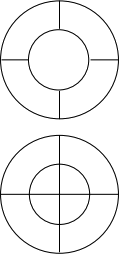
\includegraphics[width=\textwidth]{images/r-hog}
    \caption{}
    \label{fig:r-hog}
\end{wrapfigure}

As the gradient strengths vary over a wide range, based on illumination variations and foreground-background contrast, a local contrast normalization is required as a third step. This is done by grouping the histogram cells into larger blocks. The authors evaluated two grouping approaches, rectangular HOG (\acs{R-HOG}) and circular HOG (\acs{C-HOG}). \acs{R-HOG} are typical organized as $\varsigma \times \varsigma$ cell blocks (most of the time 3 or 5 blocks per direction). \acs{C-HOG} are grouped by a log-polar grid. According to the authors, at least two radial bins and four angular bins (makes a total of five to eight bins, depending if the center is also divided) as shown in figure \ref{fig:r-hog} are needed for good performance.



The authors also evaluated multiple normalization approaches to increase the detection performance.
The following approaches produced the same performance:
\begin{itemize}
	\item L2-norm $v \rightarrow v / \sqrt{||v||_2^2 + \epsilon^2}$
	\item L1-sqrt $v \rightarrow \sqrt{v / ||v||_1 + \epsilon}$
	\item L2-Hys (a L2-norm with a maximum clipping to 0.2 and a renormalization as used by Lowe \cite{Lowe2004})%$v \rightarrow \frac{\max(v / \sqrt{||v||_2^2 + \epsilon^2}, 0.2)}{\sqrt{||\max(v / \sqrt{||v||_2^2 + \epsilon^2}, 0.2)||_2^2 + \epsilon^2}}$ %TODO renormalizing 
\end{itemize}
Whilst a simple L1-norm reduced the performance by 5\% and omitting the normalization completely reduced it by 27\% according to Dalal and Triggs \cite{Dalal2005}. Another approach computes the energy of a cell and its surrounding area and uses it to normalize the cell, but also decreases the performance relative to the other approaches.

\ac{HOG} features are typically visualized by creating votes for a gradient direction based on the histogram bins of a cell. This gives a visual representation which is comprehensible from a human perspective. A sample of a \ac{HOG} representation of the lena test image can be found in figure \ref{fig:lena_hog}. Figure \ref{fig:lena_hog:8x8} shows a visualization with cells containing a $8\times8$ block of pixels and figure \ref{fig:lena_hog:32x32} a much coarser representation.

\begin{figure}[h]
    \begin{subfigure}[t]{0.3\textwidth}
        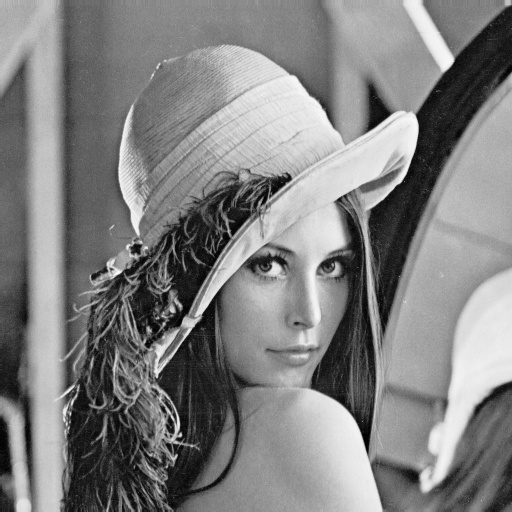
\includegraphics[width=\textwidth]{images/lena}
        \caption{Sample image in grayscale}
        \label{fig:lena_hog:lena}
    \end{subfigure}
    ~
    \begin{subfigure}[t]{0.3\textwidth}
        
\includegraphics[width=\textwidth]{images/lena_hog_8x8}
        \caption{\acs{R-HOG} representation, $8\times8$ pixels per cell}
        \label{fig:lena_hog:8x8}
    \end{subfigure}
    ~
    \begin{subfigure}[t]{0.3\textwidth}
        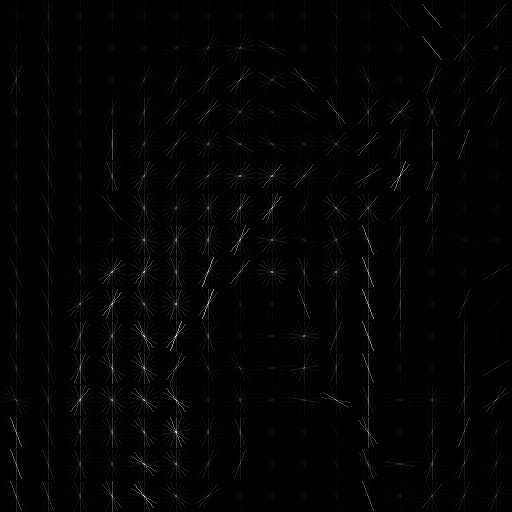
\includegraphics[width=\textwidth]{images/lena_hog_32x32}
        \caption{\acs{R-HOG} representation, $32\times32$ pixels per cell (equivalent to a downscale by 4)}
        \label{fig:lena_hog:32x32}
    \end{subfigure}
    \caption{Visualization of \ac{HOG} features}
    \label{fig:lena_hog}
\end{figure}

\ac{HOG} were initially used for pedestrian detection in static images, as Dalal and Triggs observed that the movement of individual body parts could be ignored if a general upright position is in place. Later experiments showed that it also provided good performances in other categories \cite{Malisiewicz2011}.
\subsection{\acf*{WHOG}}
\label{sec:whitened_hog}

In 2012 Hariharan, Malik and Ramanan presented a technique \cite{Hariharan2012} to reduce the background clutter captured by \ac{HOG} called \acf{WHOG}. They proposed to apply a \ac{LDA} onto the \ac{HOG} features to increase their performance as similarity measures. The idea behind the approach is to gain similar effects as using a trained \ac{SVM} to remove background information by using a \ac{LDA} model, which requires a much lower train effort compared to a \ac{SVM}. As one can see, the fence in the \ac{HOG} representation in figure \ref{fig:whitened_hog:hog} partially hides the bicycle in the front. By training a \ac{SVM} the discriminative features of the bicycles can be weightened up as shown in figure \ref{fig:whitened_hog:svm}. As the usage of a \ac{SVM} is a rather time consuming task, the authors tried technologies used in earlier computer vision algorithms like the \ac{PCA} \cite{jolliffe2002principal} and \ac{LDA} as used in \cite{ahonen2006face}. The authors observed that a down projected feature space by a simple \ac{PCA} even decreases the performance in several PASCAL \cite{Pascal2007} classes compared to unmodified \ac{HOG} features. In general, a \ac{LDA} requires labeled information about the data which is going to be separated. This would make the approach very similar to a \ac{SVM} training and classification, including the required effort (notably training of a \ac{LDA} per image category). The authors were able to show that an one-time estimated background average $\mu_0$ and covariance matrix $\Sigma$ from unlabeled windows can be used for different categories. This fact is based on the assumption that the number of any one object is small compared to the total amount of windows and therefore a object independent $\mu_0$ can be estimated.

The authors also showed that their approach is also highly comparable to an ExemplarSVM classification, but with significantly faster train and run time. 

\begin{figure}
\begin{subfigure}[b]{0.4\textwidth}
\centering
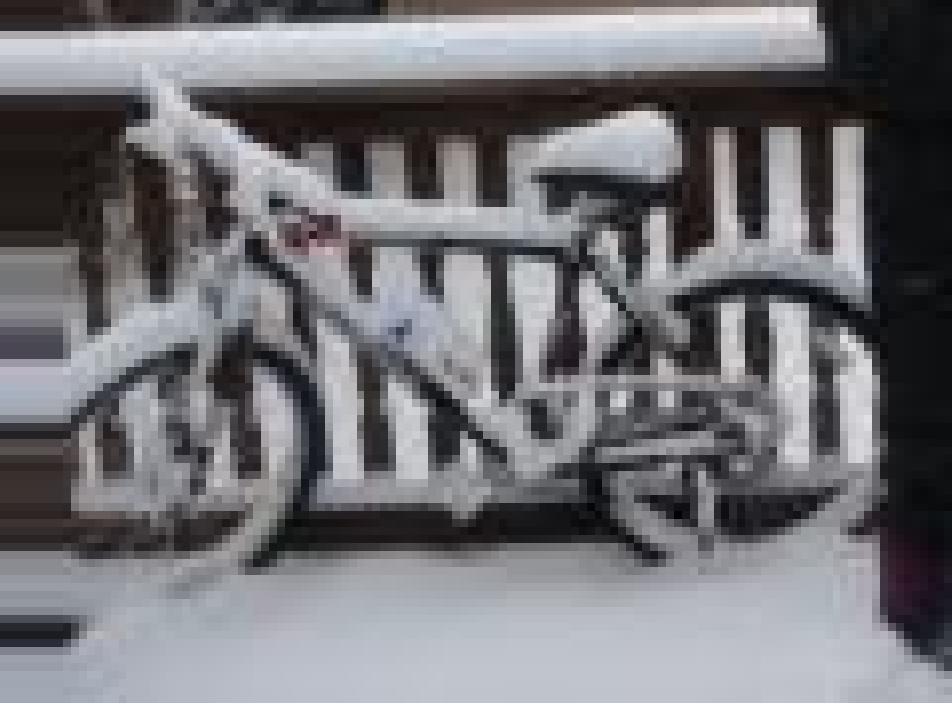
\includegraphics[width=\textwidth]{images/whitened_hog_image}
\caption[Image]{Image}
\label{fig:whitened_hog:image}
\end{subfigure}
%
\begin{subfigure}[b]{0.4\textwidth}
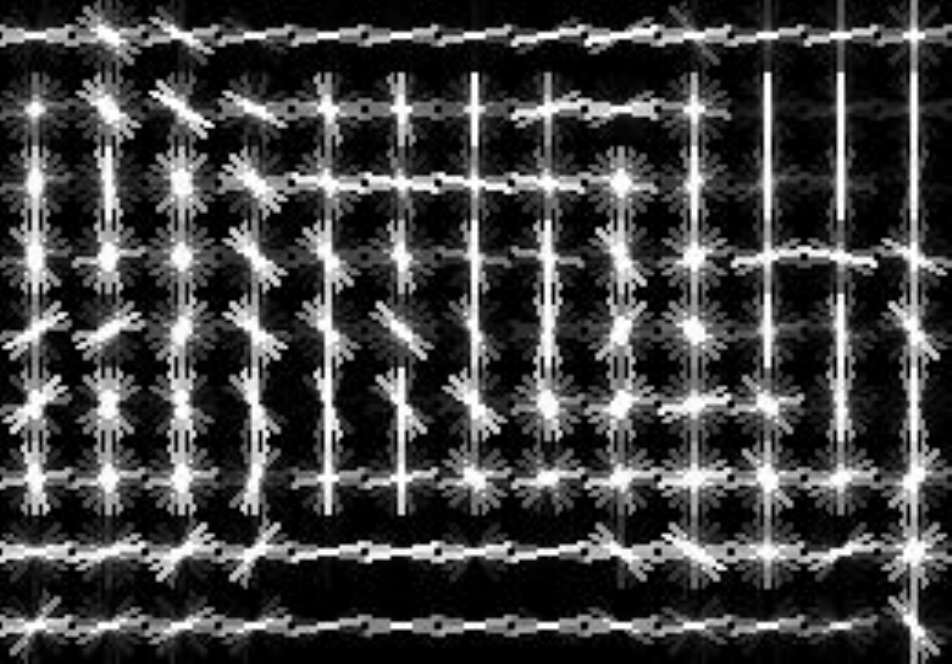
\includegraphics[width=\textwidth]{images/whitened_hog_hog}
\caption[HOG representation]{\acs{HOG} representation}
\label{fig:whitened_hog:hog}
\end{subfigure}

\begin{subfigure}[b]{0.3\textwidth}
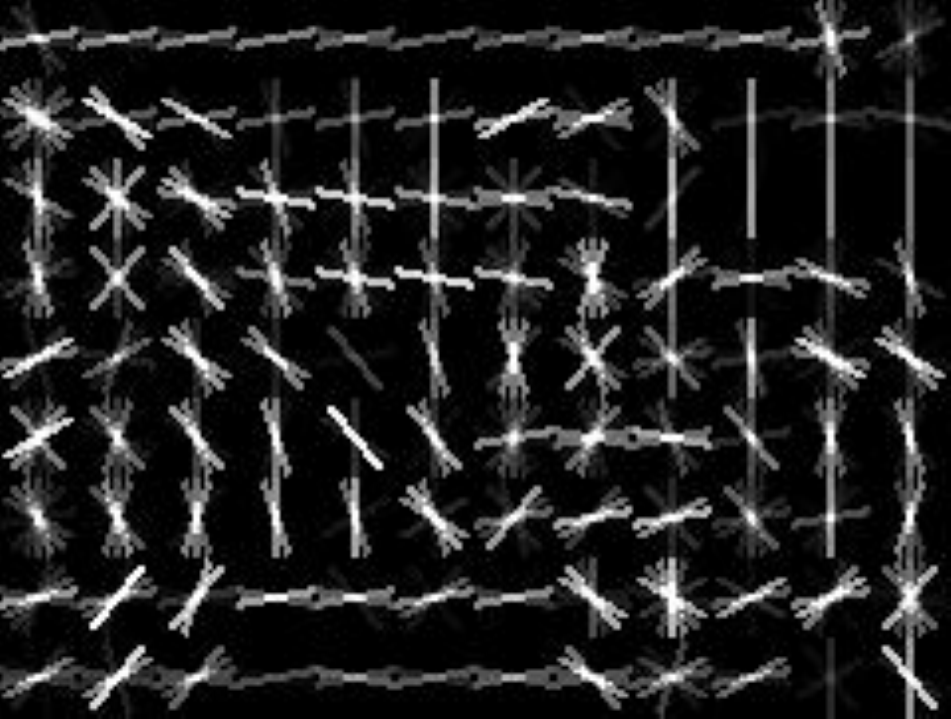
\includegraphics[width=\textwidth]{images/whitened_hog_svm}
\caption[SVM representation]{\acs{SVM} representation}
\label{fig:whitened_hog:svm}
\end{subfigure}
%
\begin{subfigure}[b]{0.3\textwidth}
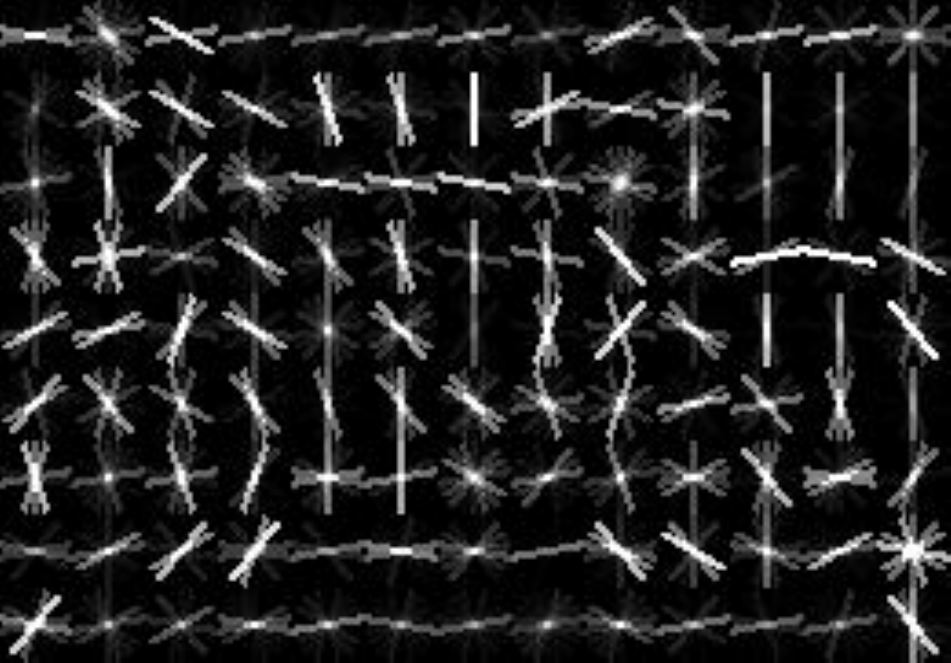
\includegraphics[width=\textwidth]{images/whitened_hog_lda}
\caption[LDA representation]{\acs{LDA} representation}
\label{fig:whitened_hog:lda}
\end{subfigure}
%
\begin{subfigure}[b]{0.3\textwidth}
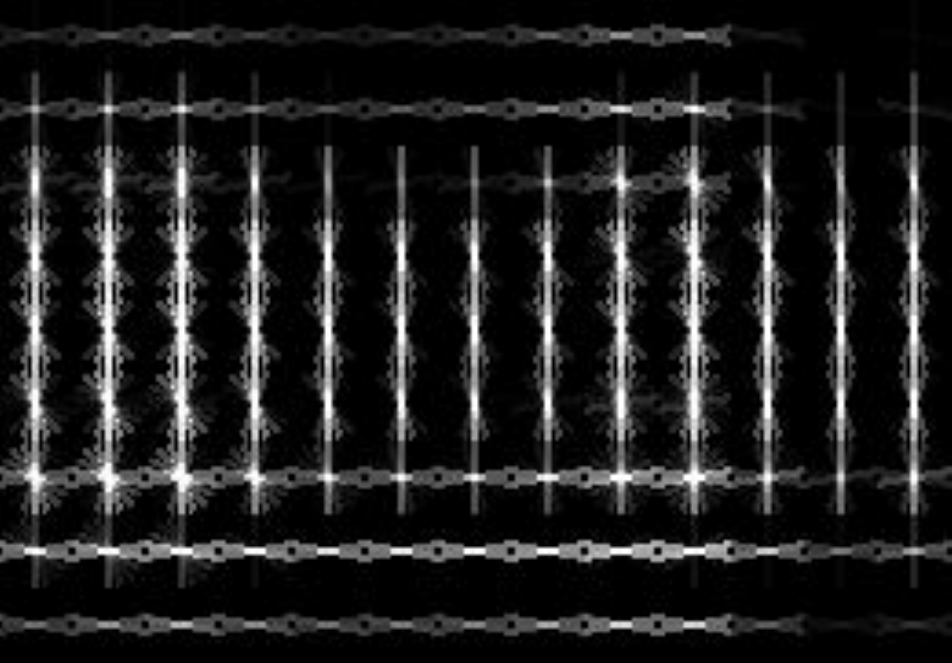
\includegraphics[width=\textwidth]{images/whitened_hog_pca}
\caption[PCA representation]{\acs{PCA} representation}
\label{fig:whitened_hog:pca}
\end{subfigure}
\caption{Bicycle in front of a fence, represented as \ac{HOG} features and weighted by different models.}
\label{fig:whitened_hog}
\end{figure}

\subsection{k-Means}
\label{sec:kmeans}

The k-means algorithm is used to partition a given set of observations into a predefined amount of $k$ clusters. The algorithm as described by \cite{macqueen1967} starts with a random set of $k$ center-points ($\mu$). During each update step, all observations $x$ are assigned to their nearest center-point (see equation \ref{eqn:kmeans_assign_step}). In the standard algorithm, only one assignment to one center is possible. If multiple centers have the same distance to the observation, a random one would be chosen.

\begin{equation}
S_i^{(t)} = \big \{ x_p : \big \| x_p - \mu^{(t)}_i \big \|^2 \le \big \| x_p - \mu^{(t)}_j \big \|^2 \ \forall j, 1 \le j \le k \big\}
\label{eqn:kmeans_assign_step}
\end{equation}

Afterwards, the center-points are repositioned by calculating the mean of the assigned observations to the respective center-points (see \eqnref{kmeans_update_step}).

\begin{equation}
\mu^{(t+1)}_i = \frac{1}{|S^{(t)}_i|} \sum_{x_j \in S^{(t)}_i} x_j
\label{eqn:kmeans_update_step}
\end{equation}

The update process reoccurs until all observations remain at the assigned center-points and therefore the center-points would not be updated anymore.

% sample images

\begin{figure}
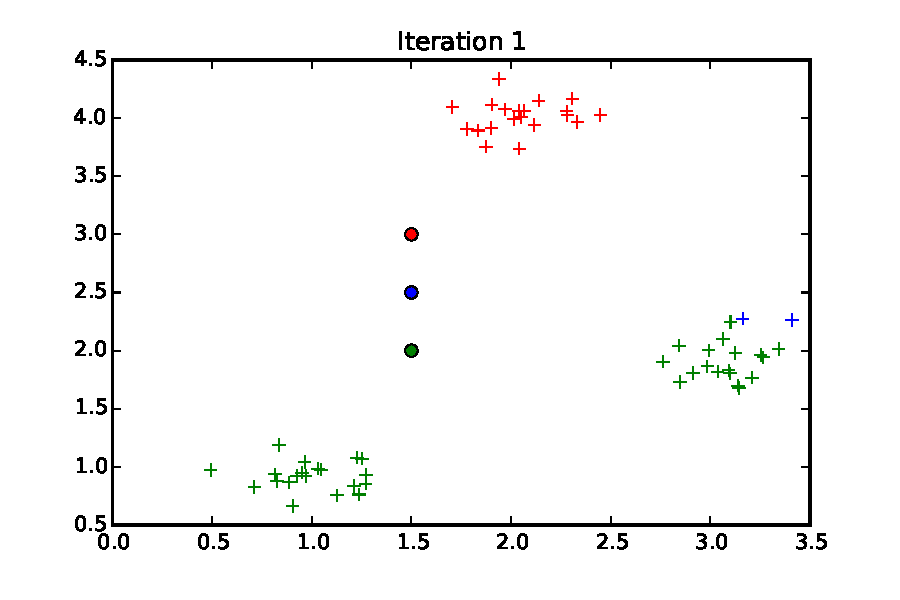
\includegraphics[width=0.6\linewidth]{images/iteration01}
\caption{k-Means: Possible initial centroid positions}
\label{fig:kmeans:iteration01}
\end{figure}

\begin{figure}
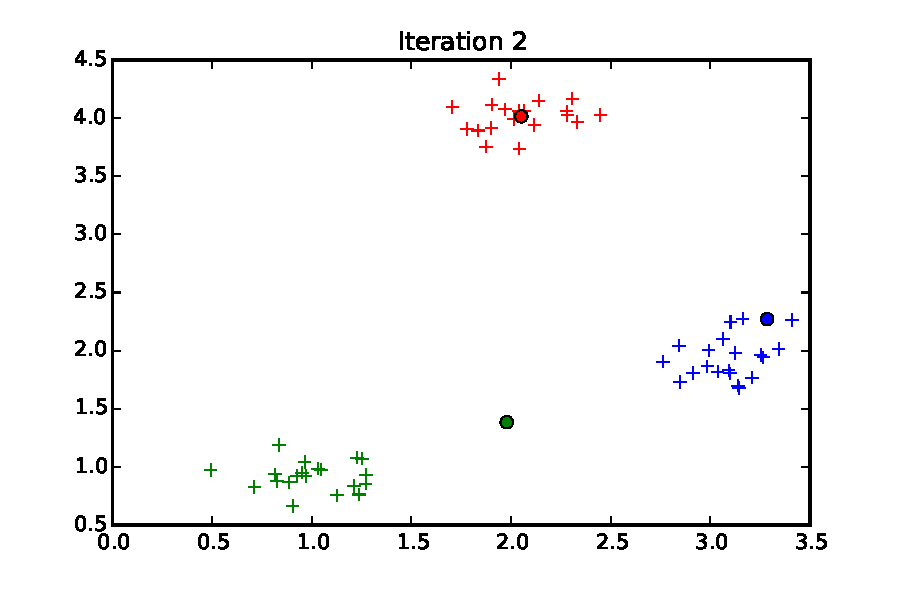
\includegraphics[width=0.6\linewidth]{images/iteration02}
\caption{k-Means: First iteration}
\label{fig:kmeans:iteration02}
\end{figure}

\begin{figure}
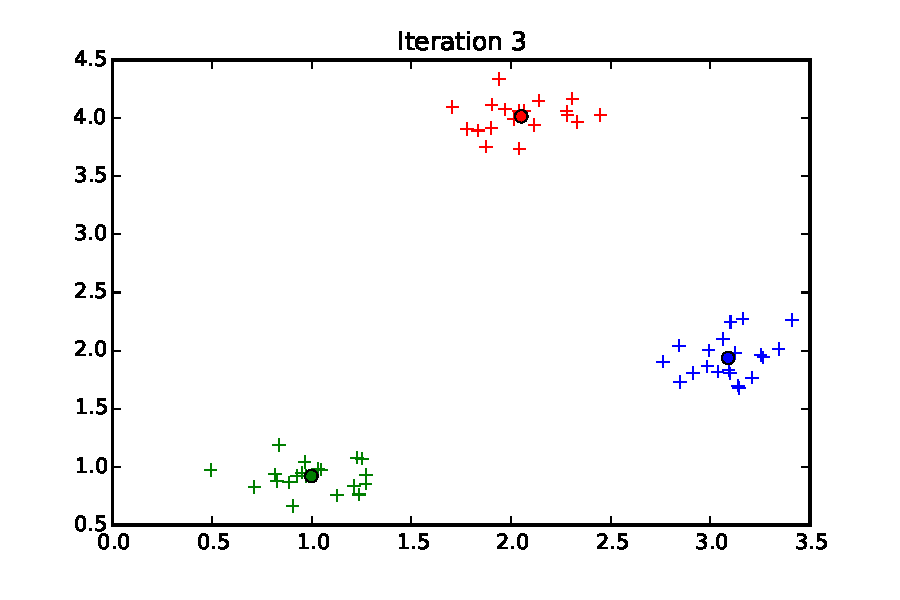
\includegraphics[width=0.6\linewidth]{images/iteration03}
\caption{k-Means: Second iteration}
\label{fig:kmeans:iteration03}
\end{figure}


This means that the k-means algorithm tries to optimize the objective function \ref{eqn:kmeans_objective_function}. As there is only a finite number of possible assignments for the amount of centroids and observations available and each iteration has to result in better solution, the algorithm always ends in a local minimum.

\begin{equation}
J = \sum_{n=1}^{N} \sum_{k=1}^{K} r_{nk} ||x_n - \mu_k||^2
\label{eqn:kmeans_objective_function}
\end{equation}

\[
\text{with } \\
r_{nk} = \begin{cases}
%1 & \text{if } k = \arg \min_j ||x_n - \mu_j||^2 \\
1 & x_n \in S_k \\
0 & \text{otherwise}
\end{cases}
\]

% minimize graph image

The main problem of k-means is its dependency on the initially chosen centroids. The centroids could end up in splitting common data points whilst other, separated points get grouped together if some of the centroids are more attracted by outliers. This points will get pulled to the same group of data points as shown in figure \ref{fig:kmeans_bad}.


\begin{figure}[h]
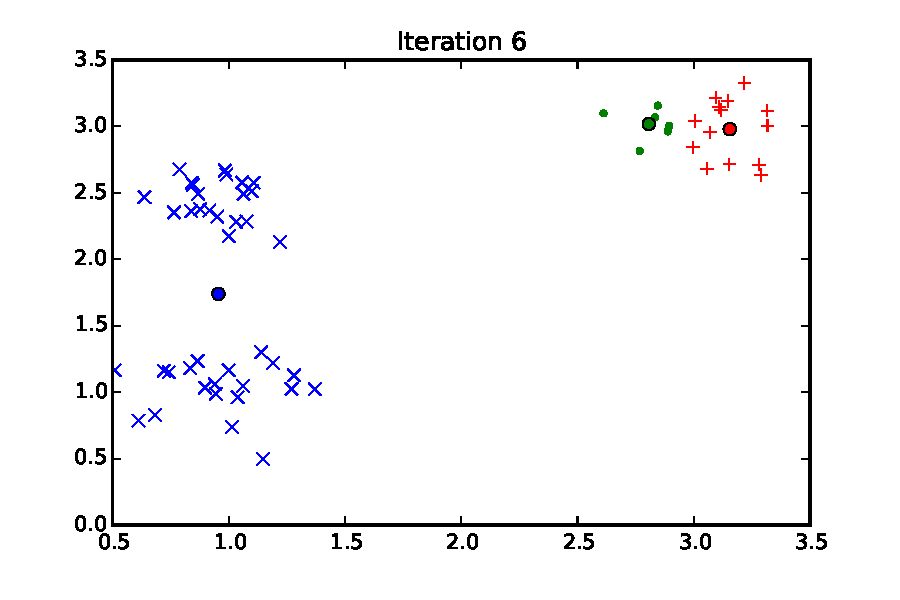
\includegraphics[width=0.6\linewidth]{images/kmeans_bad}
\caption{k-Means: Badly chosen initial center points}
\label{fig:kmeans_bad}
\end{figure}

The most common approach is to perform multiple clusterings with different start positions. Afterwards the clustering, which occurred most is considered as correct. Another, newer approach is the so called k-means++ by Arthur and Vassilvitskii \cite{Arthur:2007:KAC:1283383.1283494}. This extension to the k-means algorithm tries to distribute the initial centroids over the given data to minimize the probability of bad outcomes. The initial points are set according to the authors by the following steps

\begin{enumerate}
    \item Take uniformly a random data point from the data $X$ and mark it as centroid $c_1$
    \item Choose another centroid $c_i$ with the probability $\frac{D(x)^2}{\sum_{x \in X} D(x)^2}$ where $D(x)$ denotes the shortest distance from the data point $x$ to its closest, already chosen centroid.
    \item Repeat 2. until all $k$ initial centroids are chosen.
\end{enumerate}

Afterwards, the standard k-means algorithm as described above is performed. The authors also showed that with this initialization algorithm, k-means++ approximately can be computed in $O(\log n)$, compared to $O(n^{dk+1} \log n)$ for the standard algorithm.

\subsection{\acf{GMM}}
\label{sec:gmm}


\subsection{Fisher-Kernel}
\label{sec:fisher}

%In 2006 Florent Perronnin and Christopher Dance proposed to use Fisher kernel for image categorization \cite{Perronnin2006}. They describe Fisher kernels as a method to combine the benefits of generative and discriminative approaches (shown by \cite{jaakkola1999exploiting}). To apply Fisher kernels on visual vocabularies, they denote
%
%\begin{equation}
%\mathcal{L} (X|\lambda) = \log p(X|\lambda)
%\end{equation}
%
%With $X = \{x_t, t = 1 \dots T\}$ as a set of low-level feature vectors and $\lambda = \{w_i, \mu_i, \Sigma_i, i = 1 \dots N\}$ as a set of parameters of a \acf{GMM} ($w, \mu, \Sigma$ denote the weight, mean and covariance matrix). This corresponds to (under an independence assumption)
%
%\begin{equation}
%\mathcal{L} (X|\lambda) = \sum_{t=1}^{T} \log p(x_t|\lambda)
%\end{equation}
%
%This results in the likelihood (\eqnref{fisher_likelihood}) that a observation $x_t$ was generated by the \ac{GMM}.
%
%\begin{equation}
%p(x_t|\lambda) = \sum_{i=1}^{N} w_i p_i (x_t|\lambda)
%\label{eqn:fisher_likelihood}
%\end{equation}
%
%where the weights are constrained by \ref{eqn:fisher_weights}.
%
%\begin{equation}
%\sum_{i=1}^{N} w_i = 1
%\label{eqn:fisher_weights}
%\end{equation}
%
%The authors defined the components $p_i$ as
%
%\begin{equation}
%p_i(x|\lambda) = \frac{
%	\ 	exp \{-\frac{1}{2} (x-\mu_i)' \Sigma_{i}^{-1} (x-\mu_i)\}
%}{
%	(2 \pi)^{D/2} | \Sigma_i |^{1/2}
%}
%\end{equation}
%
%with $D$ as feature vector dimensionality and $|.|$ as determinant operator.
%% TODO
\subsection{\acf{SVM}}
\label{sec:svm}

\acfp{SVM} were initially proposed by Wladimir Wapnik and Aleksei Tscherwonenkis in 1974 \cite{vapnik1974theory}. They showed a method for classification and linear regression which becomes one of the most popular algorithms in the field of artificial intelligence \cite{russellnorvig-ai}. A \ac{SVM} is typically a binary classifier which separates multiple datapoints into two classes. A supervised \ac{SVM} training is done by placing a line (for 2-D dimensional data) or a hyperplane between two different classes by maximizing the margin between all datapoints. 
% problem
% grafik
% kernel trick
% warum
% !TeX root = ../../main.tex
 \resizebox{\textwidth}{\textwidth}{
     \tikzsetnextfilename{integral_image}
    \begin{tikzpicture}
    \foreach \x in {1,...,10} {
        \draw (\x + 0.5, 11.5) node {\x};
    }
    \foreach \x in {1,...,10} {
        \foreach \y in {1,...,10} {
            \draw (\x, \y) rectangle (\x +1, \y +1);
            \ifnumcomp{\x}{<}{2}{
                \draw[color=gray] (\x +0.5, \y +0.5) node {0};
            }{
                \ifnumcomp{\x}{<}{3}{
                    \ifnumcomp{\y}{>}{2}{
                        \draw[color=gray] (\x +0.5, \y +0.5) node {0};
                    }{
                        \draw[color=red] (\x +0.5, \y +0.5) node {1};
                    }
                }{
                    \ifnumcomp{\y}{>}{7}{
                        \draw[color=gray] (\x +0.5, \y +0.5) node {0};
                    }{
                        \ifnumcomp{\y}{>}{2}{
                            \ifnumcomp{\x}{<}{5}{
                                \draw[color=blue] (\x +0.5, \y +0.5) node {2};
                            }{
                                \ifnumcomp{\y}{>}{5}{
                                    \draw[color=blue] (\x +0.5, \y +0.5) node {2};
                                }{
                                    \ifnumcomp{\y}{>}{3}{
                                        \draw[color=orange] (\x +0.5, \y +0.5) node {5};
                                    }{
                                        \draw[color=purple] (\x +0.5, \y +0.5) node {7};
                                    }
                                }
                            }
                        }{
                            \ifnumcomp{\x}{<}{5}{
                                \draw[color=teal] (\x +0.5, \y +0.5) node {3};
                            }{
                                \draw[color=cyan] (\x +0.5, \y +0.5) node {8};
                            }
                        }
                    }
                }
            }
        }
    }
    \end{tikzpicture}
}

% !TeX encoding = UTF-8
% !TeX root = ../main.tex
% !TeX spellcheck = en_US
\chapter{Work}
\label{cha:work}

This chapter describes the experiments and approaches tried and implemented during the thesis. It should give a description about the decisions made and the problems occurred based on the decisions and implementation limitations.

\section{Extracting features}

The image feature were represented by \acf{HOG} (as described in \prettyref{sec:hog})

\section{Abstracting the feature computation}

One of the initial steps made was to find a way to represent a collection of extracted features (as taken from a part candidate or a query image). This should enable the precomputation of the image database and also create a similarity linkage right away into the stored database.

To fulfill these requirements, the decision goes to try to cluster the features with a k-means clustering (see \prettyref{sec:kmeans}) or a fisher vector representation (see \prettyref{sec:fisher}) based on a \acf{GMM} (see \prettyref{sec:gmm}).
\par
The initial experiments were used to detect if codebooks based on clustered features could be used to express similarities among different candidates. This was done by using the bicycle and car classes of the \ac{VOC2011} Image database \cite{Pascal2011}.
The clustering was initially done with 512, 1000 and 3000 k-means and 128, 256 and 384 \ac{GMM} clusters over all features extracted from the \ac{VOC2011} bicycle and car trainval image classes.
At this point all experiments were done by using normal \ac{HOG} and whiten \ac{HOG} (see \prettyref{sec:whitened_hog}) for performance comparison.
\par
The low-level \ac{HOG} implementation is provided by the Exemplar-SVM framework \cite{Malisiewicz2011}. This implementation produces a feature pyramid with $31$ dimensional features at different scales $S$.

\begin{equation}
S = \{s|s = \frac{1}{2^{0.1 * (i-1)}}; i \in \mathbb{N}; 1 \le i \le 100;\}
\end{equation}

For each level of the pyramid, the input image will be rescaled by the corresponding scale factor $s$, until no features could be extracted or the rescaled image contains less than 5 pixel per dimension.
\par
The calculated pyramid is then transfered in a list of feature vectors and their corresponding bounding boxes. This is done by combining the given features at each level of the pyramid into $5\times5$ grids and reshaping them into $775$ dimensional vectors.
As the experiments were executed with labeled bounding boxes, unnecessary features had to be removed from the list. This is achieved by specifying a pixel-wise boolean mask $M_p$ for the desired image regions. The mask will be transformed into a cell-wise $M_c$ at each scale $s$. This is done by a standard bicubic kernel convolution as in \eqnref{bicubic_kernel}.

\begin{equation}
k_x = \begin{cases}
(a+2)|x|^3-(a+3)|x|^2+1 & \text{for } |x| \leq 1 \\
a|x|^3-5a|x|^2+8a|x|-4a & \text{for } 1 < |x| < 2 \\
0                       & \text{otherwise}
\end{cases}
\label{eqn:bicubic_kernel}
\end{equation}

with $a=-0.5$ in the \MATLAB implementation\footnote{Implemented in the \textit{toolbox/images/images/imresize.m} file in the \MATLAB installation directory}. With this mask, all feature patches which are not fully covered by the mask were discarded.
\par
For the initial tests, a simple \acf{NN} approach with euclidean distances were used to compute the similarity between different codebooks.

This was done by selecting each labeled bounding box of each test image, computing the features $X$ (\ac{HOG} and whitened \ac{HOG}), assign them to the clusters by the corresponding centroids $C$ (either \ac{NN} in terms of k-means or by computing the fisher vector) and comparing it to the codebooks of the remaining image bounding boxes. The codebook values itself depend on the distances of the features to their corresponding centroids as described in \prettyref{eqn:codebook_calc}.

%TODO algorithm or formular???
%\begin{algorithm}
%	\KwIn{$X$: Features extracted from a bounding box, $C$: Cluster centroids}
%	\KwOut{$c$: codebook representing the given features}
%	\KwData{$D$: distance vector of each feature to its nearest centroid, $I$: assignment vector of each feature to its nearest centroid}
%	$D, I \gets \text{NearestNeighbourSearch}(X, C)$\;
%	
%	\ForEach{$d$ of $D$ and $i$ of $I$}{
%		$c_i \gets c_i + \frac{1}{d}$\;
%	}
%	\caption{Computing codebook from features}
%	\label{alg:codebook_calc}
%\end{algorithm}

\begin{align}
	I_j &= \arg \min_i ||X_j - C_i||_2 \\
	D_j &= \min_i ||X_j - C_i||_2 \\
	c_i &= \sum_{I_j = i} \frac{1}{D_j}
	\label{eqn:codebook_calc}
\end{align}

For a visual verification, the 15 nearest parts were shown aside to the query image. The distance between two different codebooks $c_1$ and $c_2$ was computed by the euclidean distance equation $||c_1-c_2||_2$.
%TODO beispiel bild
% searching for representative clusters (nn-iter)
For each query image, the most shared codebook dimensions and their respective patches were marked inside the images. It could be clearly seen that the patches with a comparable visual representation share the same cluster and (from a human perspective) seem to be representative for the chosen object class.
%TODO Bild mit markierung, oder auf vorheriges verweisen
To prove this assumption, an iterative \ac{NN} was implemented. It consists of several rounds, each executing a \ac{NN} search over the available patches and sorting the results. After each round, the most common codebook dimensions of the first $k$ patches were taken whilst the remaining ones were removed (set to zero) as described by \prettyref{alg:iterative_nn}.

\begin{algorithm}
	\SetKwProg{Fn}{Function}{}{end}
	\Fn{IterNearestNeighbour($q$ : query codebook, $R$ : remaining codebooks, k)}{
		\Repeat{no changes}{
			$D \gets \text{NearestNeighbourSearch}(R, q)$\;
			
			Sort $R$ based on $D$\;
			
			\tcc{$ij$ denotes dimension $i$ in codebook $j$}
			
			$S = \{i | \forall R_{ij} \ne 0; 0 < j < k\}$\;
			
			$R \gets R_{ij}$ set to $0$ if $i \notin S$\;
		}
		\Return{Sorted $R$}
	}
	\caption{Iterative \ac{NN}}
	\label{alg:iterative_nn}
\end{algorithm}

By using this algorithm, it could be shown that the most representative patches were assigned to the same clusters, as more similar objects are pulled together at each iteration.
%TODO bilder fuer verschiedene iterationen 

\par
% maintaining location information (parts)
As the reduction of several feature vectors to a single codebook for a whole bounding box eliminates the locational information, the implementation was extended to maintain some locational information by splitting the bounding box in several parts and computing a codebook for each of them. Afterwards, these codebooks are concatenated, which means that the size of a representative codebook for a whole bounding box is calculated by $numberOfParts * numberOfDimensions$. This change brought additional performance gains in terms of detecting similar parts, but also increased the memory usage significantly. During the rest of the experiments, the bounding boxes were either split into a two-by-two grid (as it seemed to be the best mix of performance gain and memory usage) or left complete for later comparisons.

\section{Scoring the part candidates}

% svm

As the direct comparison via a \ac{NN} approach did not provided the desired performance and also resulted in a time consuming task if the amount of codebooks increases, another approach was required. One possible solution for detecting similar vectors is a \ac{SVM} based classifier (for a more detailed description about \acp{SVM} see \prettyref{sec:svm}). In this particular case a C-SVC classifier was trained \cite{boser1992training} \cite{cortes1995support}.
%In this particular case a one-vs-call classifier was used. In this type only one classifier is trained to determine if a given vector is part of one class or part of all other possible classes.
The positive class is represented by the query codebook, whilst all other classes are represented by a previously collected list of codebooks. To generate this list, a set of sliding windows were calculated for each image in the database based on \algref{calc_windows}.

\begin{algorithm}
    \KwIn{$I$: image}
    \KwOut{calculated windows}
    $w_I \gets \text{width of }I$\;
    $h_I \gets \text{height of }I$\;
    $S \gets \{s^2 | s \in \mathbb{N}, s \le 10 \}$\;
    $x \gets \{1, 11, 21, 31,\dots, w_I\}$\;
    $y \gets \{1, 11, 21, 31,\dots, h_I\}$\;
    \Repeat{$w_w >= w_I$ or $h_w >= h_I$ or no elements left in $S$}{
        $currentScale \gets \text{next element of }S$\;
        $w_w \gets 32 * currentScale$\;
        $h_w \gets 32 * currentScale$\;
        
        \ForEach{Combination $x_i, y_i$ of $x$ and $y$}{
            Add window $x_i, y_i, x_i + w_w, y_i + h_w$ to the list\;
        }
    }
    \caption{Calculation of sliding windows}
    \label{alg:calc_windows}
\end{algorithm}

With this list, all feature patches are assigned to these windows where their center is placed in. For each window, a codebook is calculated by \eqnref{codebook_calc}. The resulting list of codebooks is stored and loaded during the \ac{SVM} training and used as the negative training set. The \ac{SVM} training was done by the libsvm library \cite{Chang:2011:LLS:1961189.1961199} by using the \texttt{svmtrain} function. The parameters for the training are the same as for the ExemplarSVM library \cite{Malisiewicz2011} (see \tabref{libsvm_train_params}).

\begin{table}
    \begin{tabular}{|l|l|}
        \hline
        \textbf{Parameter} & \textbf{Value} \\ 
        \hline
        SVM-Type           & C-SVC \\ 
        \hline
        Kernel-Type        & Linear ($u^T*v$) \\ 
        \hline
        Cost ($C$ of C-SVC)  & $0.01$ \\ 
        \hline
        Weight of positive sample ($weight*C$) & $50$ \\ 
        \hline
    \end{tabular}
    \caption{libsvm parameters}
    \label{tab:libsvm_train_params}
\end{table}

Other assignment methods were also evaluated, including multi assignments like assigning a feature to every window were a corner is located in, or to every window which contains a minimum amount of the patch (e.g. 30\% of its area). These approaches did not provide enough performance gain in comparison to the computational overhead. Another approach was the usage of the bottom right corner, which obviously led to the fact that the detection candidates were slightly shifted to the bottom right compared to an optimum detection. 

In the first place, the classification function provided by libsvm\footnote{\texttt{svmpredict(\dots)}} was used. With an increasing amount of codebooks which have to be classified by the \ac{SVM}, the function toked a big part of the computation time. By replacing the function with the \MATLAB implementation ($codebooks * (svm_{vectors}^T * svm_{coefficents}) - svm_{\rho}$) (see \prettyref{lst:matlab_svm_predict}), the computation time could be reduced from approximate 150 seconds to 3 seconds with 250,000 codebooks (5,000 windows in 50 images).


\begin{lstlisting}[caption={\MATLAB variant of svmpredict},label=lst:matlab_svm_predict]
weights = m.SVs' * m.sv_coef;

if size(codebooks, 2) == size(weights, 1)
    scores = codebooks * weights - m.rho;
else
    scores = codebooks' * weights - m.rho;
end
nans = isnan(scores);
debg('%d NaNs produced!', sum(nans))
scores(nans) = -999;
\end{lstlisting}

\section{Reducing the computational overhead}

% integral image
During the shift from the initial tests involving the usage of labeled bounding boxes to the actual requirement of finding parts inside of image databases, the amount of computational overhead increased significantly as it requires to compute sliding windows on each image in the database and their codebooks respectively.

Therefore the idea came up to precompute the codebooks and only load them at runtime for comparison. One solution would be to compute a set of possible windows and their codebooks. At query time the best matching window ratios could be loaded and compared to the query codebook. Unfortunately was the performance dramatically decreased with this approach.

The second solution was to create integral images based on codebooks. Integral images were described by Viola and Jones in 2001 \cite{viola2001rapid}. Such images are created by summing up all pixel values from the top left to the bottom right (or any other diagonal direction). The advantage of this approach is the possibility to compute a sum value for a rectangular area by summing and subtracting the values of the four corners as described in \figref{integral_image}. 

\begin{figure}
\begin{tikzpicture}
\draw (0,0) rectangle (5,5);
\draw[fill=blue] (0,5) rectangle (2,4);
\draw (1.75, 4.25)  node[white] {$A$};
\draw[fill=red] (2,5) rectangle (4,4);
\draw (4.25, 4.25)  node{$B$};
\draw[fill=yellow] (0,4) rectangle (2,3);
\draw (1.75, 2.75)  node{$C$};
\draw[fill=green] (2,4) rectangle (4,3);
\draw (4.25, 2.75)  node{$D$};
\end{tikzpicture}
\caption[Sum of area in integral image]{The sum of all values in the green area could be computed by $A+D-(C+B)$. $A$ is the sum of all pixels in the blue area, $B$ the sum of the pixels in the blue and the red areas, $C$ the sum of all pixels in the blue and yellow areas, $D$ of the green, red, blue and yellow respectively}
\label{fig:integral_image}
\end{figure}

The difference to \cite{viola2001rapid} is that one pixel at a time is represented by a complete codebook, therefore an integral image per codebook dimension has to be computed. The source image is created by adding the inverse distance of each feature patch center to its nearest cluster centroid to the corresponding codebook dimension. Afterwards, a cumulative sum over the two image axes is computed. The benefit of using integral images is that at runtime, every possible window could be computed by four reads (the corners), one sum and two subtractions between the codebooks. This reduced the computational time at the query stage to 1-2 seconds with a $500\times375$ image, 1000 codebook dimensions and 5000 windows with a 2-by-2 grid.

The downside is the memory usage, which increased dramatically. For example, a $500 \times 375 \times 1000$ integral image requires with the double datatype at least 1.4 gigabytes of data (without any meta information stored aside by matlab). The 50 images test database required therefore at least 70 gigabytes of RAM storage during the query. This also led to the problem of the time required to load the whole database. By storing it in the \MATLAB 7.3 file format, which effectively is a slightly modified HDF5 \cite{hdf5}, the program requires in average 900 seconds to load the whole database from a network shared filesystem.

This method also enabled the extraction of the query codebook from an image contained in the database without any feature or codebook computations. The reduced computational effort during the query phase consist therefore in extracting the query codebook from the database, training of the \ac{SVM}, calculating the sliding windows, extracting the codebook for each window in each image and scoring the codebooks by the trained \ac{SVM}.
% no libsvm classify

\section{Optimizing the score output}

%TODO non max suppression

The experiments showed that the \ac{SVM} output does not provide a clear separation threshold to identify positive candidates over all images in the database. The scores varied between -2 and 1 for the best matching candidates. As the candidates were most of the time correctly ordered by their visual similarity to the query image, this would not be a problem under the assumption that every image contain at least one area which is similar to the query image part. In this case, the scores could be normalized at an image level, which means that significant higher scores compared to the arithmetic mean are considered positive, whereas scores near the mean or lower are considered negative. %TODO bild von score histogram
As one will see in \figref{score_histogram}, this would fit for the most pictures used during the testing. The majority of windows is located at the same score, whereas windows with a score above the mean are closely located to the desired image part.
% gaussian fit + rho adjust
This additional normalization obviously increases the computation effort as it had to be done separately for each image in the database (after computing the scores for each window in the image). Therefore an approximation was applied by normalizing the scores in relation to the query image. To normalize the scores, a Gaussian curve is fitted onto the scored query image windows. By shifting the curve by $3\sigma$ into the direction of the highest scores, the relevant (positive) scores where pulled up near to one, whereas the negative scores get pushed down to zero. The resulting curve is then applied to all scores. This approximated normalization enabled us to produce comparable scores and therefore exclude whole images from the query results.

Another approach was to create a per image $svm_\rho$ value (comparable to the mean threshold) to orientate the scores at a common center point, but it turned out that the effort were to high compared to the performance gain.

After the score computation and normalization, a non maximum suppression was applied to minimize the output of similar, near located windows.
During the experiments, two non maximum suppression techniques were used and evaluated.

The first one is constructed by the union of the areas to compare (\ref{eqn:nonmax_union})

\begin{equation}
\frac{\text{area}(A \cap B)}{\text{area}(A \cup B)}
\label{eqn:nonmax_union}
\end{equation}

This technique computes the ratio between the common and total area of two bounding boxes $A$ and $B$. If this ratio has a value higher than $0.5$, the bounding box $B$ would be removed from the result list.

The second technique is based on \eqnref{nonmax_min}. This variant removes much more bounding boxes if they are enclosed by others, as only the area of smallest bounding box is used as the denominator. The previous technique removes only enclosed bounding boxes which are at least half as big as their enclosing boxes.

\begin{equation}
\frac{\text{area}(A \cap B)}{\min(\text{area}(A), \text{area}(B))}
\label{eqn:nonmax_min}
\end{equation}

The current algorithm produced the best results with the second technique, as it reduces the repetition of many positive windows showing only a single bicycle wheel. As they would not cover 50\% of the window enclosing the whole bicycle, they appear as new matches in the result list by using the first technique. Depending on the query image, it could be useful to switch between the suppression techniques as it could be desired to get smaller matches enclosed by a bigger one (for example children in front of their parents).

\section{Reducing the memory usage}

After optimizing the detection performance, the memory usage was still to high to provide an useful alternative/boosting algorithm to the ExemplarSVM algorithm. To minimize the memory overhead, several approaches were developed and evaluated. These approaches include different storage mechanisms as kd-tree, spares matrices or plain index-value pairs and also different search and reconstruction strategies.

\subsection{Sparse matrices}

One approach is to use sparse matrices as provided by the \MATLAB framework\footnote{\url{https://de.mathworks.com/help/matlab/ref/sparse.html}}. The usage seemed to be very promising, as partial inspections of the integral images showed that approx. 70\% of the cells in a $512\times500\times375$ matrix are filled with zeros.

It showed that the \MATLAB implementation of sparse matrices is restricted to two-dimensional matrices, it is therefore required to reduce the amount of dimensions of the matrix at store time and restore the original format at runtime, or transform the required coordinates into a single index. As the internal representation of an image consists of four matrix dimensions (scale range, codebook dimensions, width, height), a matrix will be transformed into a matrix of the form $CB \times N$ whereas $CB$ is the amount of codebook dimensions and $N$ the product of the image width, height and number of scale ranges included in this matrix (usually one per saved \MATLAB file). The corresponding source code could be seen in \lstref{storage_method_sparse} in line 171. The variable \verb|si| represents the current scale ranges which will be saved. A complete reconstruction to the original, internal representation could be done with \lstref{reconstruct_sparse_matlab}. This is done by converting the sparse matrix into a full matrix containing the zero values. The new matrix is then reordered into its original four dimensional representation.

\begin{lstlisting}[firstnumber=165,caption={Sparse storage method (get\_codebook\_integrals.m)},label=lst:storage_method_sparse]
I2 = I(si, :, :, :);
Is = size(I2);
integrals(si, fi).I_size = Is;
if params.naiive_integral_backend
    integrals(si, fi).I = I2;
elseif params.integral_backend_matlab_sparse
    integrals(si, fi).I = sparse(squeeze(I2(:, :, :)));
\end{lstlisting}

\begin{lstlisting}[firstnumber=29,caption={Sparse reconstruction by \MATLAB (getCodebookIntegrals.m)},label=lst:reconstruct_sparse_matlab]
I = full(integralImg.I);
I = reshape(I, integralImg.I_size);
\end{lstlisting}

The matrices are stored in a \MATLAB file with the 7.3\footnote{A comparison table could be found at \url{https://de.mathworks.com/help/matlab/ref/save.html\#input_argument_version} (visited on 10/12/2015)} file format (required to store variables with more than two gigabytes of data).
For example the representation of the pascal image \textit{2007\_008932.jpg} containing feature patches with a maximum size of $86\times86$ pixels and 512 codebook dimensions results in a total \ac{RAM} size of 768,001,438 bytes (or 732.4 megabytes). The saved \MATLAB file occupies 6,325,415 bytes (6 megabytes) of disk space.
Stored as a sparse matrix the data is reduced to 423,905,670 bytes (404.3 megabytes or 55\%) in \ac{RAM}. After saving to a file, a size of 22,612,163 bytes (21.6 megabytes) still remains. Compared to the na\"{\i}ve (saving the matrices as is) storage method it requires 16,286,748 bytes more (15.5 megabytes or 357\%) disk space. The reason for this storage overhead could probably be found in the mandatory compression which comes with file formats greater or equal to version 7.0. For the na\"{\i}ve format, the compression can benefit from the low entropy coming from the high amount of zeros which exists in a sequential ordering. In contrast to the sparse variant, which have to compress multiple lists of coordinates and their corresponding values. Besides the fact that disk storage is a cheap resource nowadays, it also affects the loading time as more data has to be loaded. Although the decompression time could be reduced as a much lesser compression ratio was achieved. Together with the additional matrix reconstruction described above, a small speedup was still achieved whilst the memory usage was reduced by 50\%.

\subsection{Reconstructing from changing points}

As the internal representation is based on integral images, additional information can be interfered from on specific points in the matrix. Integral images are constructed by summing up values from the top left to the bottom right. This means that as long as no further points exists in the source image, the most current value is carried on until the next point is found. The example in \figref{integral_image_interference} shows and describes the behavior. As one can see, the minimum required information to construct a full integral image are the values at the points $(2,9)$, $(3,4)$, $(5,6)$ and $(5,8)$. In contrast to the sparse matrix approach, only 4 points have to be stored compared to 58 points.

Obviously the computation effort during the query search increases as the integral image would had to be computed at runtime. By sorting the points according to the sum of their coordinate values, the computation overhead could be reduced as the amount of cells which have to be summed up decreases with every point processed.
%TODO timings + memory

%\begin{lstlisting}[firstnumber=229,caption={Coordinate based storage method (get\_codebook\_integrals.m)},label=lst:storage_method_coordinate]
%[cb, x, y] = ind2sub(Is(2:end), find(remaining));
%coords = [x, y, cb];
%
%sum_values = coords(:, 1) + coords(:, 2);
%[~, idx] = sort(sum_values);
%coords = coords(idx, :);
%scores = scores(idx, :);
%
%integrals(si, fi).coords = coords;
%integrals(si, fi).scores = scores;
%\end{lstlisting}

To find a trade-off between low memory usage and computation effort, another approach came up. In this approach every changing value in the integral image is stored instead of the original values. In the current example the points $(2,9)$, $(3,4)$, $(3,9)$, $(5,6)$, $(5,8)$ and $(5,9)$ would be selected. By storing the additional points, which were created at the intersection points of the original ones, we are able to reconstruct the full matrix by taking the list of points, sorting them by the sum of their coordinates and writing one point at a time from its position to the bottom right. In the current example the list would be sorted as \mathlist{(3,4), (5,6), (2,9), (3,9), (5,8), (5,9)}. In the first step the point $(3,4)$ would be selected and its value ($2$) would be written to the bottom right as shown in \figref{integral_image_interference2:point1}. The second step selects point $(5,6)$ and write its value $5$ in the same way as before.
This technique will be applied to all points in the list until the integral image is fully reconstructed.
The speed up comparing to the previous approach is based on the fact that no memory read from any cell has to be made and no arithmetic instruction has to be executed. The limiting factor in this case is ability to write values fast at specific positions in \ac{RAM}.
%TODO timings + memory

\begin{figure}
\begin{subfigure}{.5\textwidth}
    \resizebox{\textwidth}{\textwidth}{
        \begin{tikzpicture}
        \foreach \x in {1,...,10} {
            \draw (\x + 0.5, 11.5) node {\x};
        }
        \foreach \y in {10,...,1} {
            \draw (0.5, 11.5 - \y) node {\y};
        }
        \foreach \x in {1,...,10} {
            \foreach \y in {1,...,10} {
                \draw (\x, \y) rectangle (\x +1, \y +1);
                \ifnumequal{\x}{5}{
                    \ifnumequal{\y}{5}{
                        \draw[color=red] (\x +0.5, \y +0.5) node {3};
                    }{
                        \ifnumequal{\y}{3}{
                            \draw[color=red] (\x +0.5, \y +0.5) node {2};
                        }{
                            \draw[color=gray] (\x +0.5, \y +0.5) node {0};
                        }
                    }
                }{
                    \ifnumequal{\x}{2}{
                        \ifnumequal{\y}{2}{
                            \draw[color=red] (\x +0.5, \y +0.5) node {1};
                        }{
                            \draw[color=gray] (\x +0.5, \y +0.5) node {0};
                        }
                    }{
                        \ifnumequal{\x}{3}{
                            \ifnumequal{\y}{7}{
                                \draw[color=red] (\x +0.5, \y +0.5) node {2};
                            }{                    
                                \draw[color=gray] (\x +0.5, \y +0.5) node {0};
                            }
                        }{
                            \draw[color=gray] (\x +0.5, \y +0.5) node {0};
                        }
                    }
                }
            }
        }
        \end{tikzpicture}
    }
    \caption{Source image}
    \label{fig:integral_image_interference:source_image}
\end{subfigure}%
\begin{subfigure}{.5\textwidth}
    \resizebox{\textwidth}{\textwidth}{
        \begin{tikzpicture}
        \foreach \x in {1,...,10} {
            \draw (\x + 0.5, 11.5) node {\x};
        }
        \foreach \x in {1,...,10} {
            \foreach \y in {1,...,10} {
                \draw (\x, \y) rectangle (\x +1, \y +1);
                \ifnumcomp{\x}{<}{2}{
                    \draw[color=gray] (\x +0.5, \y +0.5) node {0};
                }{
                    \ifnumcomp{\x}{<}{3}{
                        \ifnumcomp{\y}{>}{2}{
                            \draw[color=gray] (\x +0.5, \y +0.5) node {0};
                        }{
                            \draw[color=red] (\x +0.5, \y +0.5) node {1};
                        }
                    }{
                        \ifnumcomp{\y}{>}{7}{
                            \draw[color=gray] (\x +0.5, \y +0.5) node {0};
                        }{
                            \ifnumcomp{\y}{>}{2}{
                                \ifnumcomp{\x}{<}{5}{
                                    \draw[color=blue] (\x +0.5, \y +0.5) node {2};
                                }{
                                    \ifnumcomp{\y}{>}{5}{
                                        \draw[color=blue] (\x +0.5, \y +0.5) node {2};
                                    }{
                                        \ifnumcomp{\y}{>}{3}{
                                            \draw[color=orange] (\x +0.5, \y +0.5) node {5};
                                        }{
                                            \draw[color=purple] (\x +0.5, \y +0.5) node {7};
                                        }
                                    }
                                }
                            }{
                                \ifnumcomp{\x}{<}{5}{
                                    \draw[color=teal] (\x +0.5, \y +0.5) node {3};
                                }{
                                    \draw[color=cyan] (\x +0.5, \y +0.5) node {8};
                                }
                            }
                        }
                    }
                }
            }
        }
        \end{tikzpicture}
    }
    \caption{Integral image}
    \label{fig:integral_image_interference:integral_image}
\end{subfigure}%
\caption{The source image in \subref{fig:integral_image_interference:source_image} contains values at the positions $(2,9)$, $(3,4)$, $(5,6)$ and $(5,8)$. As shown in \subref{fig:integral_image_interference:integral_image} their values expand to the bottom right. Even if the amount of zero values decreased, the matrix contain still a high percentage of repetitions.}
\label{fig:integral_image_interference}
\end{figure}

\begin{figure}
\begin{subfigure}{.5\textwidth}
    \resizebox{\textwidth}{\textwidth}{
        \begin{tikzpicture}
        \foreach \x in {1,...,10} {
            \draw (\x + 0.5, 11.5) node {\x};
        }
        \foreach \y in {10,...,1} {
            \draw (0.5, 11.5 - \y) node {\y};
        }
        \foreach \x in {1,...,10} {
            \foreach \y in {1,...,10} {
                \draw (\x, \y) rectangle (\x +1, \y +1);
                \ifnumcomp{\x}{<}{3}{
                    \draw[color=gray] (\x +0.5, \y +0.5) node {0};
                }{
                    \ifnumcomp{\y}{>}{7}{
                        \draw[color=gray] (\x +0.5, \y +0.5) node {0};
                    }{
                        \draw[color=blue] (\x +0.5, \y +0.5) node {2};
                    }
                }
            }
        }
        \end{tikzpicture}
    }
    \caption{Reconstructing point $(3,4)$}
    \label{fig:integral_image_interference2:point1}
\end{subfigure}%
\begin{subfigure}{.5\textwidth}
    \resizebox{\textwidth}{\textwidth}{
        \begin{tikzpicture}
        \foreach \x in {1,...,10} {
            \draw (\x + 0.5, 11.5) node {\x};
        }
        \foreach \x in {1,...,10} {
            \foreach \y in {1,...,10} {
                \draw (\x, \y) rectangle (\x +1, \y +1);
                \ifnumcomp{\x}{<}{3}{
                    \draw[color=gray] (\x +0.5, \y +0.5) node {0};
                }{
                    \ifnumcomp{\y}{>}{7}{
                        \draw[color=gray] (\x +0.5, \y +0.5) node {0};
                    }{
                        \ifnumcomp{\y}{<}{6}{
                            \ifnumcomp{\x}{>}{4}{
                                \draw[color=orange] (\x +0.5, \y +0.5) node {5};
                            }{
                                \draw[color=blue] (\x +0.5, \y +0.5) node {2};
                            }                                                    
                        }{
                            \draw[color=blue] (\x +0.5, \y +0.5) node {2};
                        }                      
                    }
                }
            }
        }
        \end{tikzpicture}
    }
    \caption{Reconstructing point $(5,6)$}
    \label{fig:integral_image_interference2:point2}
\end{subfigure}%
\caption{Reconstructing integral image from intersection points}
\label{fig:integral_image_interference2}
\end{figure}

The fourth approach tried to achieve an additional reduction of the writing cycles. This is done by storing additional points, which are selected by scanning the integral image row by row. Each time a value change is detected, the point is added to the list. In the example the complete list would be noted as \mathlist{(3,4), (3,5), (3,6), (5,6), (3,7), (5,7), (3,8), (5,8), (2,9), (3,9), (5,9), (2,10), (3,10), (5,10)}. In the reconstruction phase, the algorithm jumps at the first point for each row and writes its value to the right until he reaches the next point in the list. Now the new value is written to right until the next point is reached and so forth.
%TODO timings + memory

The fifth approach skips the reconstruction completely and tries to find any value by searching in the list of intersection values from the third approach. In the initial implementation, the scores were stored aside to their x, y and codebook dimension coordinates ($img_x$, $img_y$ and $img_{codebook}$ respectively). The actual search consisted of three steps. In the first step, all coordinates and values are selected which correspond to the lower or equal x values compared to the query x value ($query_x$). Within the subset all values belonging to $img_y \le query_y$ are selected. The resulting subset is scanned from lower to higher coordinates (sorted by $img_x$, $img_y$ and $img_{codebook}$) and will fill a codebook based on the $img_{codebook}$ and score values.

As one may notice this represents more or less multiple linear searches, which has to be done by every requested codebook at a specific point. To speedup the search a binary searching algorithm based on kd-trees were implemented. %TODO binary search, kd-tree
Instead of filtering by the x and y coordinates first and filling the codebook with the last changed values, the filtering for this approach was reversed. Every integral image is represented by as many kd-trees as codebook dimensions exist. If one codebook dimension is never used throughout the while image, the corresponding tree will be empty. Each of the remaining trees consist of two matrices. The first matrix contains three rows with as many columns as unique x coordinates for this codebook dimension exist. The first row contains the current x coordinate, the second the starting index for the second matrix and the third row the end index for the second matrix. The second matrix consists of two rows. One containing all y coordinates and the other all scores.

When searching a value for a specific codebook dimension at a specific point, the kd-tree which corresponds to the codebook dimension is selected. Within the first matrix the highest x value lower or equal to $query_x$ is searched and the second matrix is cut to the start and end indices extracted from the first matrix. Within this smaller matrix the highest y value lower or equal to $query_y$ is searched and the corresponding score is used as the codebook dimension value. Both searches can be done by a binary search approach in $O(\log_2 N)$. Additionally, most of the searches will be canceled early, as either the codebook dimension is empty, the $query_x$ is outside of the x values or $query_y$ is outside of the y values. %TODO nachweis????
%TODO timings + memory

%\begin{lstlisting}[firstnumber=179,caption={KD-Tree storage method (get\_codebook\_integrals.m)},label=lst:storage_method_kdtree]
%remaining = I2 ~= 0;
%
%I2 = I2(remaining);
%scores = I2(:);
%if params.use_kdtree
%    [cb, x, y] = ind2sub(Is(2:end), find(remaining));
%    % sort order: y x cb
%    coords = [cb, x, y];
%    cb = unique(cb);
%    cblen = length(cb);
%    if cblen > 0
%        tmptree = alloc_struct_array(cblen, 'x', 'y');
%        parfor ci=1:cblen
%            dim = cb(ci);
%            if ci == 1 || ci == cblen || mod(ci, 100) == 0
%                debg('[%4d/%04d] Dimension %d', ci, cblen, dim);
%            end
%            cs = coords(:, 1) == cb(ci);
%            x = coords(cs, 2);
%            y = coords(cs, 3);
%            s = scores(cs);
%            ux = unique(x);
%            data2 = zeros([length(ux) 3], 'uint32');
%            data2(:, 1) = ux;
%            data3 = zeros([length(y) 2]);
%            from = 1;
%            to = 0;
%            for xi=1:length(ux)
%                xs = x == ux(xi);
%                sxs = sum(xs);
%                if sxs
%                    to = to + sum(xs);
%                    data3(from:to, 1) = y(xs);
%                    data3(from:to, 2) = s(xs);
%                    data2(xi, [2 3]) = [from, to];
%                    from = to+1;
%                end
%            end
%            tmptree(ci).x = data2;
%            tmptree(ci).y = data3;
%        end
%        tree = alloc_struct_array(Is(2), 'x', 'y');
%        tree(cb) = tmptree;
%    else
%        tree = alloc_struct_array(Is(2), 'x', 'y');
%    end
%
%    %tree = create_kd_tree(cb, tree);
%    integrals(si, fi).tree = tree;
%\end{lstlisting}

% kd - tree
% sparse matrix
% overwrite
% sum

\section{The framwork}


\chapter{Experiments and Results}
\label{cha:experiments}

As multiple approaches were developed during the thesis, several experiments were required. These experiments can be categorized into 

\begin{itemize}
\item memory usage
\item file size
\item time required to
    \begin{itemize}
    \item load the database
    \item extract codebooks from the database
    \item do a complete query run
    \end{itemize}
\item detection performance
\end{itemize}

To test the loading times, the different storage mechanisms were each tested with 512 and 1000 codebook dimensions. Together with the different mechanism, this results in total to 14 unique combinations. Each combination loads the same database containing 50 images with an average size of 476x391 pixels\footnote{The list of PASCAL ids can be found in the appendix \ref{apx:images50}}. It should be noted that all mechanisms result in the same integral images at runtime or at least provide the same results on extraction.


\begin{figure}
\begin{subfigure}[t]{0.5\textwidth}
\centering
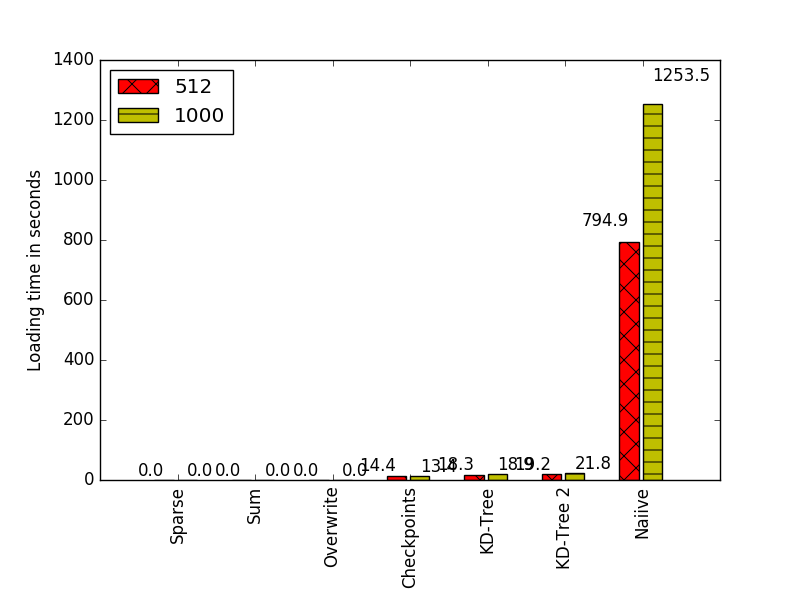
\includegraphics[width=\linewidth]{images/loading_time}
\caption{Loading times of all database storage backends.}
\label{fig:loading_all}
\end{subfigure}%
%
\begin{subfigure}[t]{0.5\textwidth}
\centering
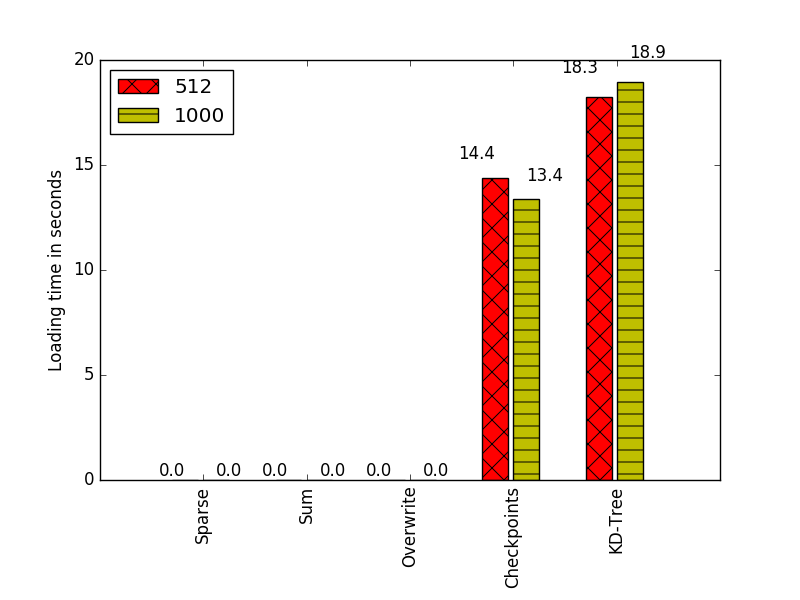
\includegraphics[width=\linewidth]{images/loading_time_2}
\caption{Loading times of all database storage backends except the na\"{\i}ve and sparse ones.}
\label{fig:loading_except_naiive}
\end{subfigure}

\caption{Loading times of the different database storage backends.}
\end{figure}


As one can see in \figref{loading_all} the na\"{\i}ve approach (which stores the complete matrices) obviously requires an unusable amount of time to load the database. One reason that the loading time does not have a linear dependency on the codebook size, is that \MATLAB uses a compression for files with version 7 and above and the possibility for empty codebook entries or similar entries increases for higher dimensional vectors. The approach which stores only a sparse representation with zero values removed, was much faster, but still requires to much time to load compared to the whole computing time of the ExemplarSVM algorithm (85 seconds for 50 images). In \figref{loading_except_naiive} one can see the loading times without the na\"{\i}ve and sparse approaches as they are too close to each other compared to these two approaches.


\begin{figure}
\centering
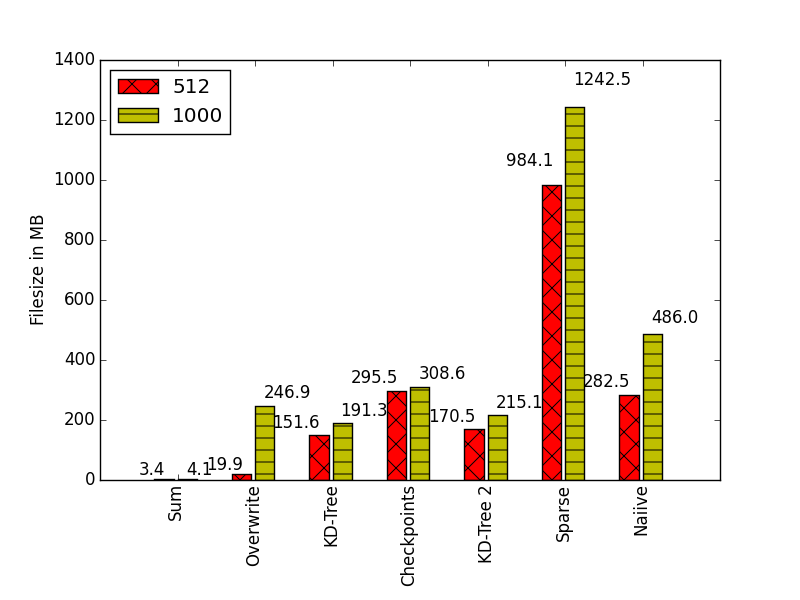
\includegraphics[width=0.7\linewidth]{images/file_size}
\caption[File sizes of the different storage backends]{File sizes of the different storage backends. These are mostly based on the compression of the data and have the most impact on network file storages.}
\label{fig:file_sizes}
\end{figure}

\Figref{file_sizes} shows the file sizes of the different techniques. As one may notice, the \MATLAB sparse representation of the database requires much more space on the filesystem compared to the na\"{\i}ve approach, but loads faster. This is because the internal representation of the sparse matrices was not as small compressed as the full matrices, possibly mainly because the amount of consecutive data is much reduced. Obviously, the compressed matrices have to be uncompressed during load, which requires more time than loading the bigger file of sparse matrices. As the compression is mandatory for \MATLAB files with version 7 and up\footnote{\label{footnote:matlab_files}As described on \url{https://de.mathworks.com/help/matlab/ref/save.html?refresh=true} (visited 11/06/2015)} and version 7.3 is required due to the large variable sizes\footnoteref{footnote:matlab_files}, this behavior can not be circumvented.

\begin{figure}
\begin{subfigure}[t]{0.5\textwidth}
\centering
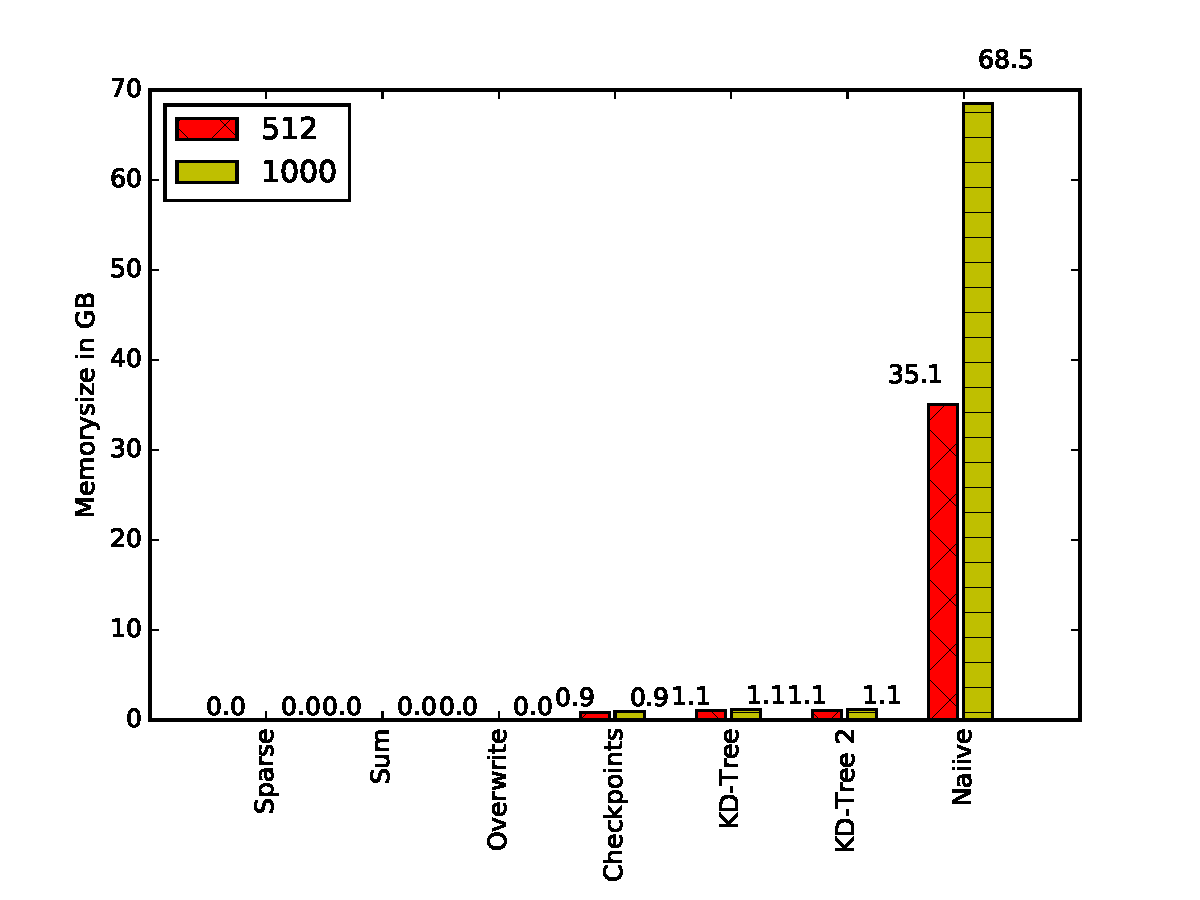
\includegraphics[width=\linewidth]{images/mem_size}
\caption{All backends}
\label{fig:memory_usage}
\end{subfigure}%
%
\begin{subfigure}[t]{0.5\textwidth}
\centering
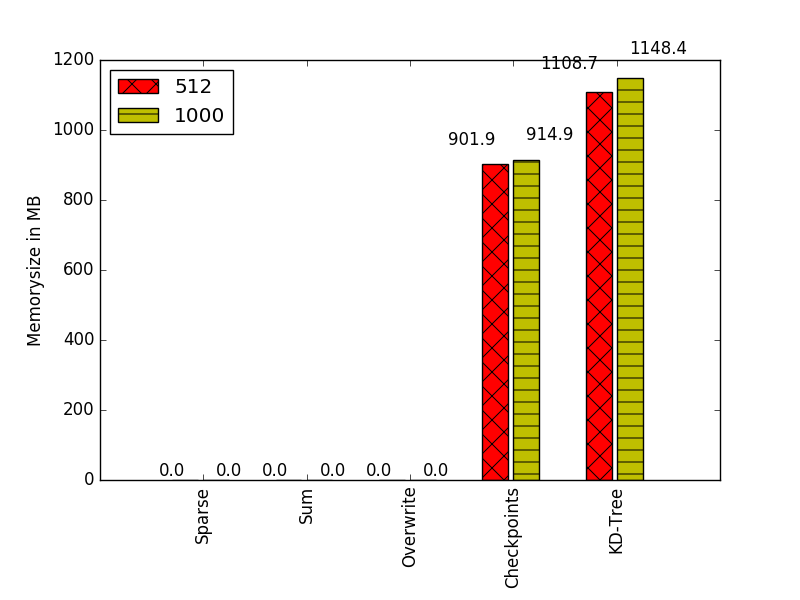
\includegraphics[width=\linewidth]{images/mem_size2}
\caption{All backends except the na\"{\i}ve and sparse ones.}
\label{fig:memory_usage2}
\end{subfigure}

\caption{Memory usage of the different storage backends.}
\end{figure}

The memory usage of the different techniques in \ac{RAM} is shown in \figref{memory_usage}. It has to be noted that some of the techniques (namely the summation and overwrite) require the reconstruction of the original integral images. This increases the memory usage during runtime, but (in contrast to the na\"{\i}ve technique) only for one image at a time (when it is queried). The required size depends on the information, which is needed to reconstruct every possible extraction point. As the summation techniques calculates the integral image at runtime, it requires the least stored information. The implementation of the sparse storage mechanism allows only to omit cells with a zero value and therefore has to store all cells, which are in the bottom left of the first filled cell for a codebook dimension. The kd-Tree variants, compared to the checkpoints variant, require some additional meta information to build up the tree.

To complete the comparison between the different mechanisms, the time required to extract a complete set of windows from an image was measured. The computation of the window list was based on \textit{2008\_004363.jpg} with the bounding box $x_{min} = 102, y_{min} = 178, x_{max} = 344, y_{max} = 336$. This results into 4784 windows. As one can see in \figref{extract_time}, the live reconstruction of the integral image by using the summation or overwrite technique are clearly the most time consuming ones.

%TODO describe figure!!!!

\begin{figure}
\centering
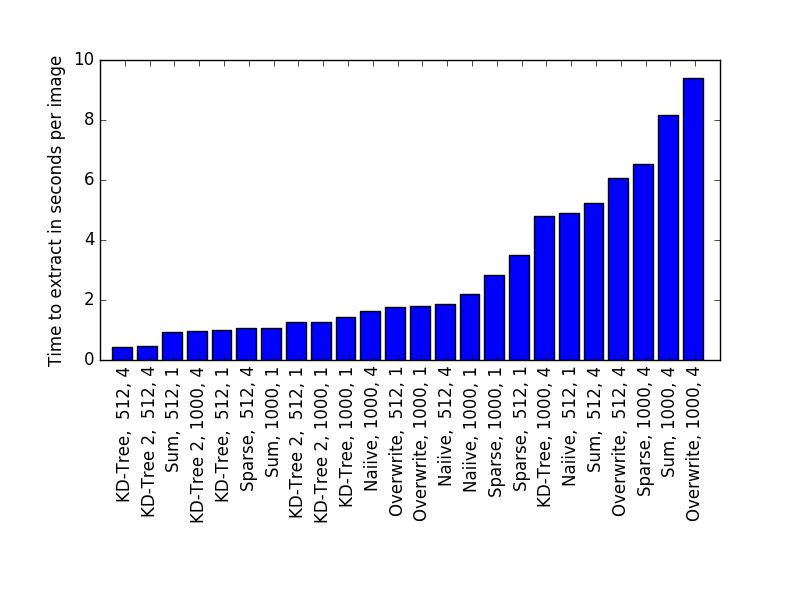
\includegraphics[width=\linewidth]{images/extract_times}
\caption[Extraction times of different parameter combinations.]{Extraction times of different parameter combinations based on the average of a 50 image database.}
\label{fig:extract_time}
\end{figure}

As the ExemplarSVM does not load precomputed data, except of the negative features for the \ac{SVM} training, it was not possible to compare it with the different parts of the tested approaches. Instead the total processing time is used.
With the initial implementation, which uses a sliding window algorithm with a fixed 10 pixel shift, the amount of searched windows (between 4000 and 7500, depending on the query image) is much higher compared to the searched windows in the ExemplarSVM algorithm (limited to 400). This obviously results in a high processing time for all configurations as one can see in \figref{processing_time_windows}.

\begin{figure}
\centering
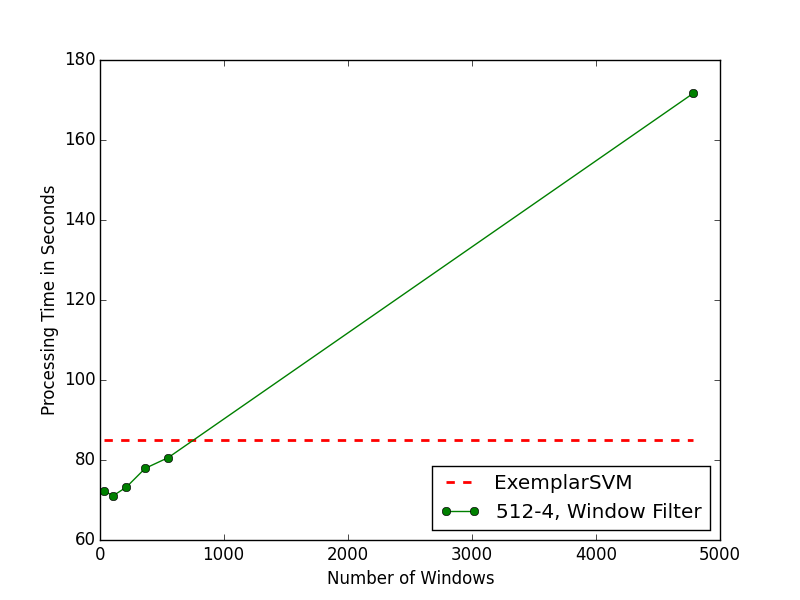
\includegraphics[width=0.7\linewidth]{images/window_comparison-512-4-filtered}
\caption[Window comparison]{Comparison of the processing time of different amount of sliding windows. The red dashed line represents the processing time of an ExemplarSVM search with the same database and query part.}
\label{fig:processing_time_windows}
\end{figure}


Further experiments used an implementation, which shifts the windows based on their size. This reduces the amount of windows and therefore increases the processing speed as shown in \figref{processing_time_windows}.
As it obviously also reduces the number of hypotheses, the possibility to find a perfect match decreases. To see the relationship between the amount of windows and the detection performance, multiple runs with different configurations and window slide settings were done.

\begin{figure}
\begin{subfigure}{\textwidth}
\centering
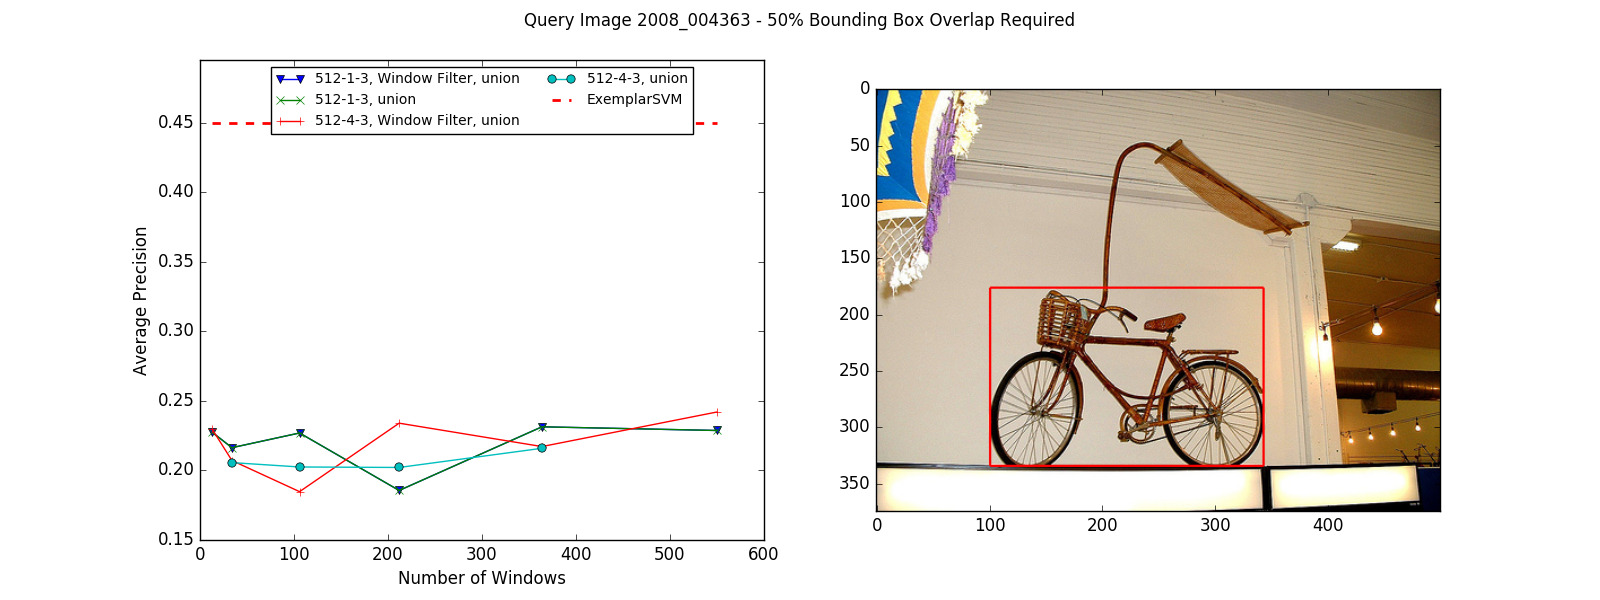
\includegraphics[width=\textwidth]{images/db1_window_comparison-2008_004363}
\end{subfigure}

\begin{subfigure}{\textwidth}
\centering
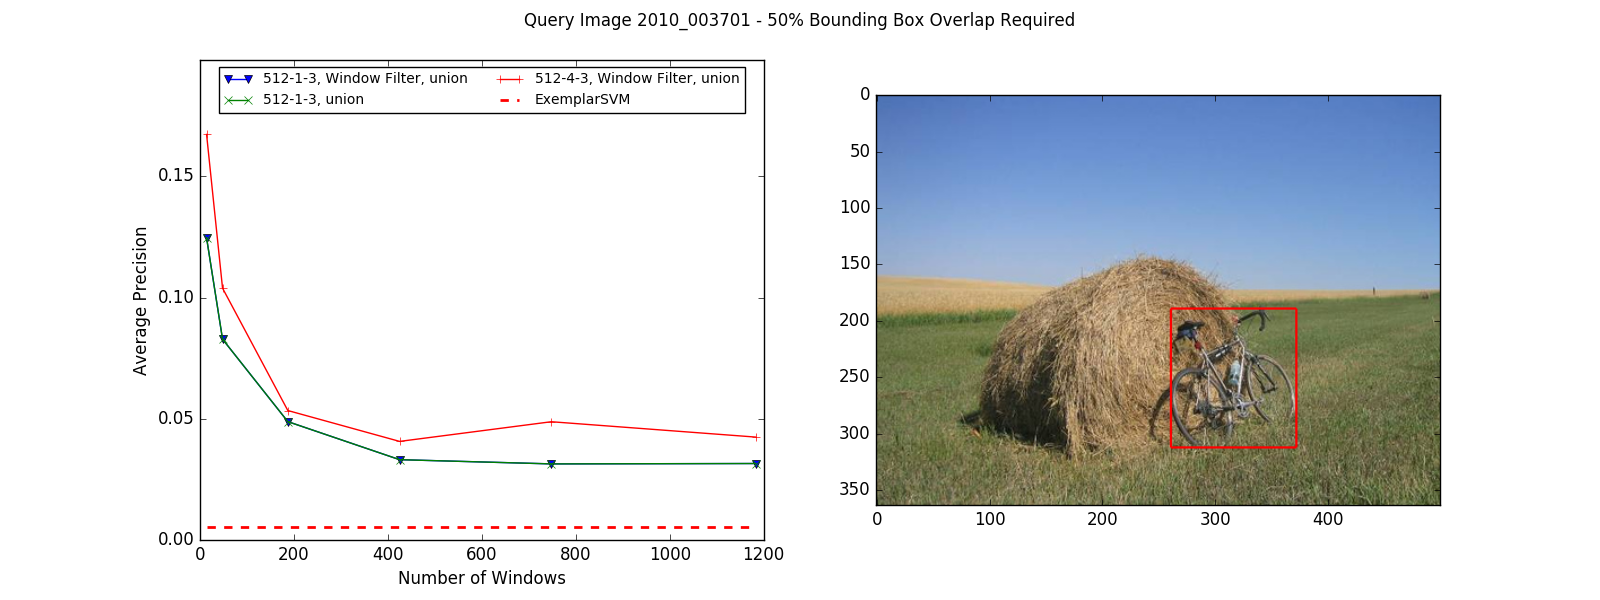
\includegraphics[width=\textwidth]{images/db1_window_comparison-2010_003701}
\end{subfigure}
\caption[Performances of querying with 2008\_004363 and 2010\_003701 with different techniques and window amounts]{Performances of querying with 2008\_004363 and 2010\_003701 with different techniques and window amounts. 512-4-3 represents 512 clusters, windows divided into 4 parts, database splitted into 3 scale ranges.}
\label{fig:performance_query_params}
\end{figure}


The tests with the files from appendix \ref{apx:images50} provided a performance, which comes near to the ExemplarSVM. Additionally, some of the query images performed much better compared to the ExemplarSVM algorithm (\figref{performance_query_params}). Based on the significantly performance differences between ExemplarSVM and the tested approaches on some test images, together with the fact that the results could not be directly correlated to the chosen parameters, the assumption arises that there is some bias in the test set. This bias results in a behavior, which always prefers windows enclosing a large portion of an image. Combined with the fact that (the randomly chosen) test images contain many images with bicycles nearly of the image size, this results in similar performance rates for different bicycle queries. To add more variance to the test set, more randomly chosen images have been added to get 234 images in total (97 bicycle and 137 non-bicycle images).

By using this image set, the performance slightly decreased (as expected) (\figref{db2_window_comparison-ALL} compared to \figref{db1_window_comparison-ALL}). Additionally the parameter combination which was expected to provide the best results (4 parts with window prefilter) jumps from the worst to the best. This could be either explained by a measurement error, or because of the increased amount of negatives in the dataset. Therefore result in more penalties if the detection is not accurate enough. The performance compared to the search time is similar to the 50 image dataset, although some of the parameter combinations (primarily 4 parts, single scale range) took more time in average (per processed image in the database) than the ExemplarSVM. This could be explained by the increased general size of the database and the higher amount of data as all different input scales were loaded together.

For the third iteration of the tests, the first 2500 images of the the \ac{VOC2011} bicycle validation dataset were used. This time, the performance gap between the ExemplarSVM and the different approaches increased and the processing time of all parameter combinations was higher than the ExemplarSVM variant. As this also corresponds to the increased loading time of the database (the processing alone was significant lower than the ExemplarSVM in previous experiments), this could be mitigated by loading smaller chunks of the database. This allows to separate the I/O operations from the CPU intensive tasks. Due to the limited time, this adjustment was not implemented.


\begin{figure}
\centering
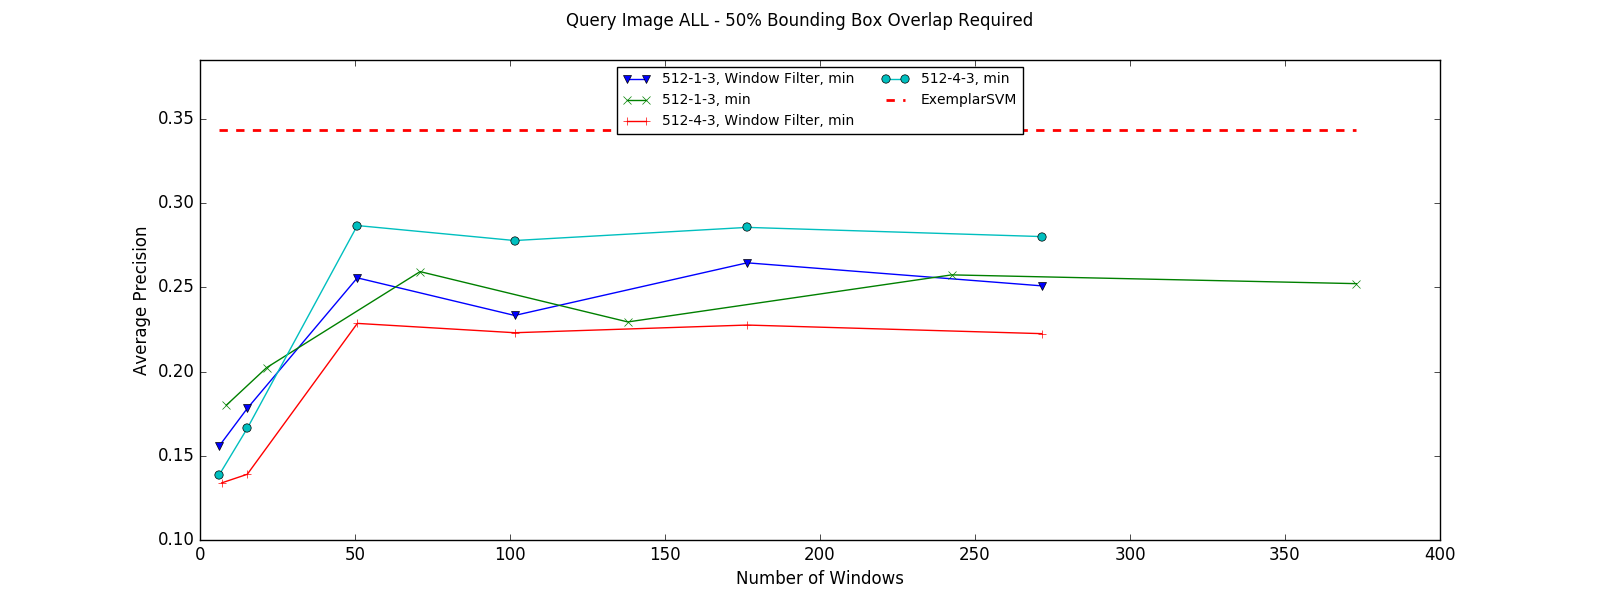
\includegraphics[width=\linewidth]{images/db1_window_comparison-ALL}
\caption{Averaged detection performance of different windows compared to ExemplarSVM (50 images)}
\label{fig:db1_window_comparison-ALL}
\end{figure}


\begin{figure}
\centering
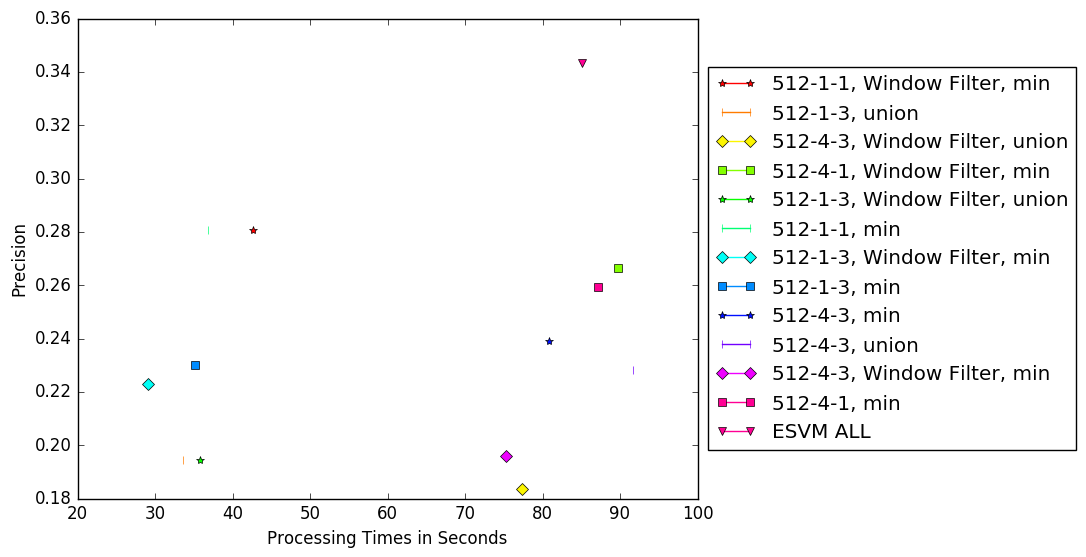
\includegraphics[width=0.7\linewidth]{images/db1_t_vs_p-ALL}
\caption{Performance versus search time (50 images)}
\label{fig:db1_t_vs_p-ALL}
\end{figure}

\begin{figure}
\centering
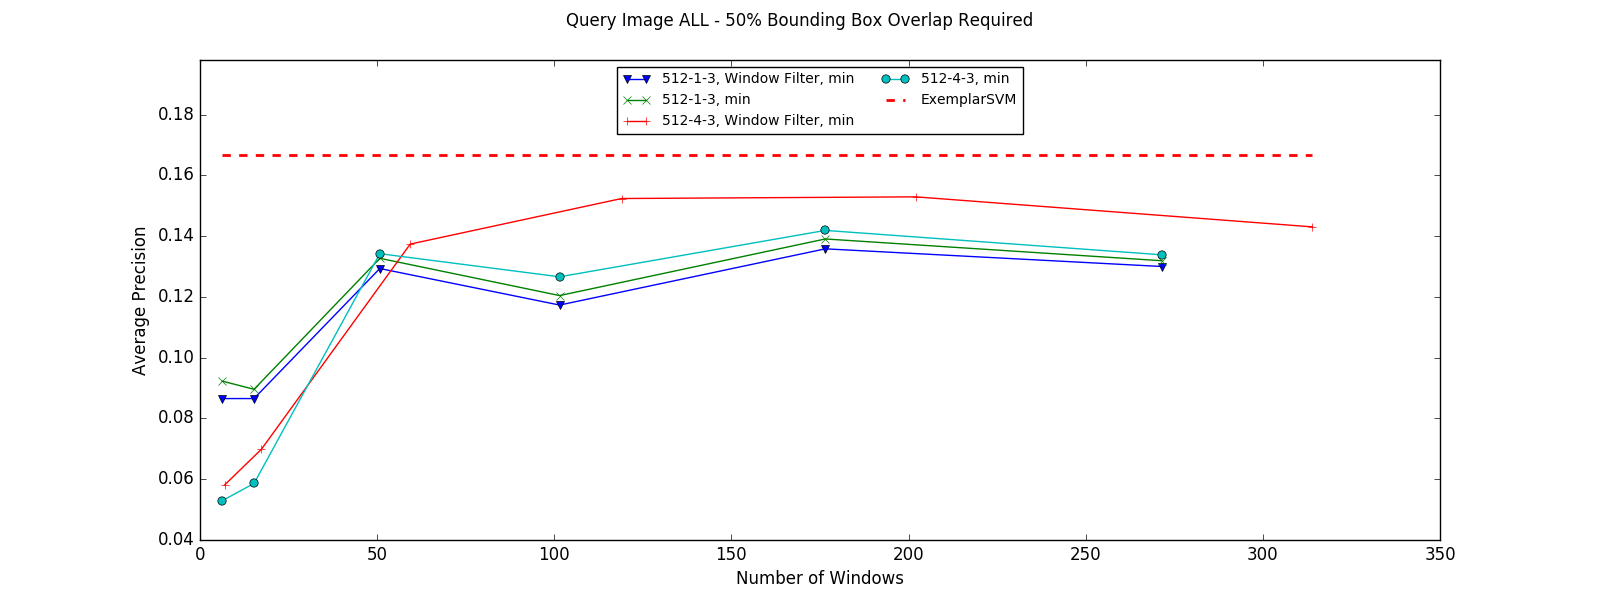
\includegraphics[width=\linewidth]{images/db2_window_comparison-ALL}
\caption{Averaged detection performance of different windows compared to ExemplarSVM (100 images)}
\label{fig:db2_window_comparison-ALL}
\end{figure}


\begin{figure}
\centering
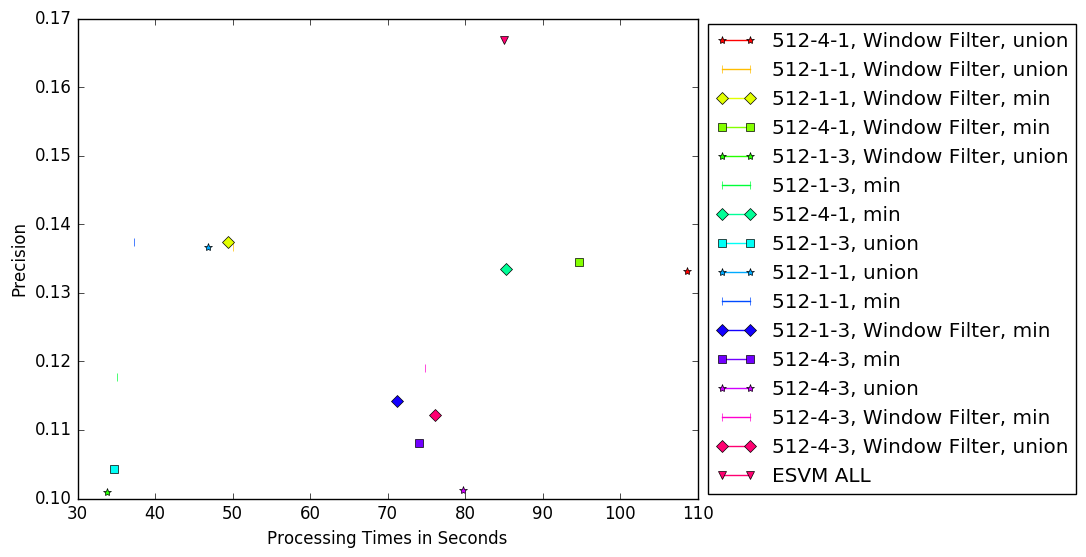
\includegraphics[width=0.7\linewidth]{images/db2_t_vs_p-ALL}
\caption{Performance versus search time (100 images)}
\label{fig:db2_t_vs_p-ALL}
\end{figure}

\begin{figure}
\centering
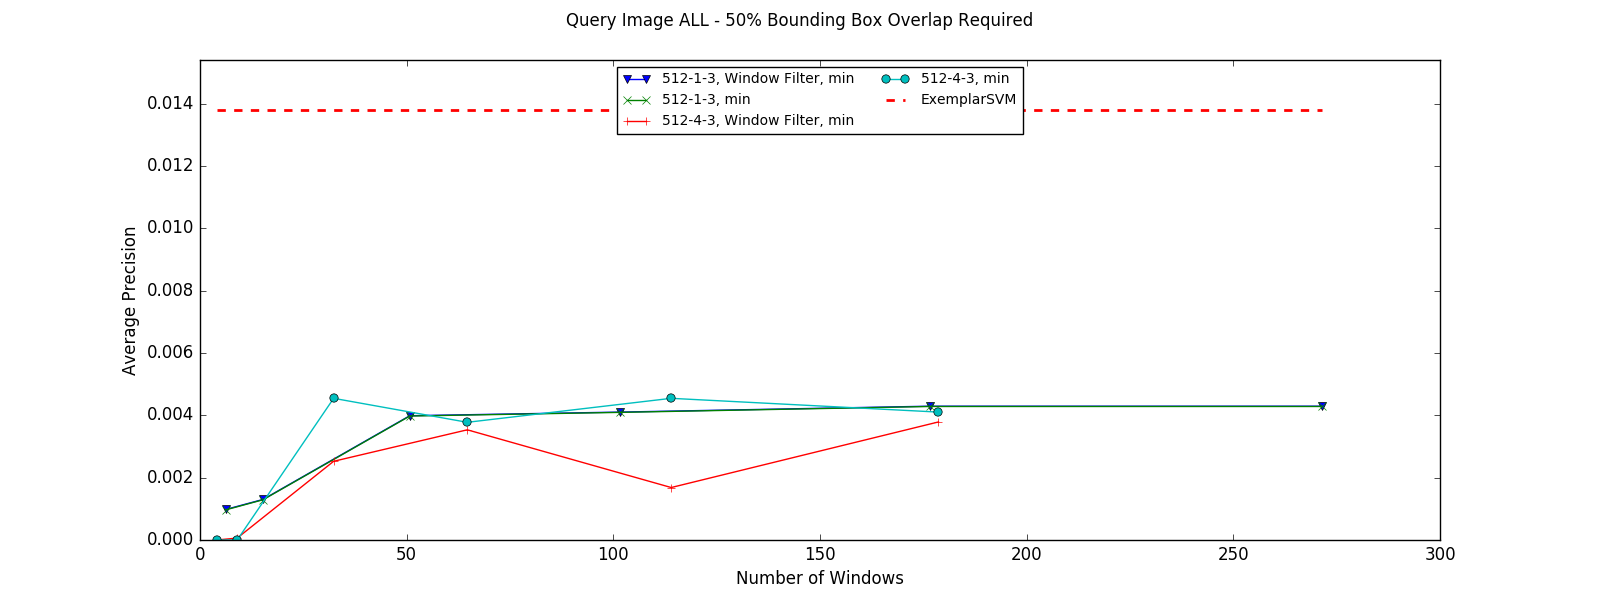
\includegraphics[width=\linewidth]{images/val_window_comparison-ALL}
\caption{Averaged detection performance of different windows compared to ExemplarSVM (2500 images)}
\label{fig:val_window_comparison-ALL}
\end{figure}


\begin{figure}
\centering
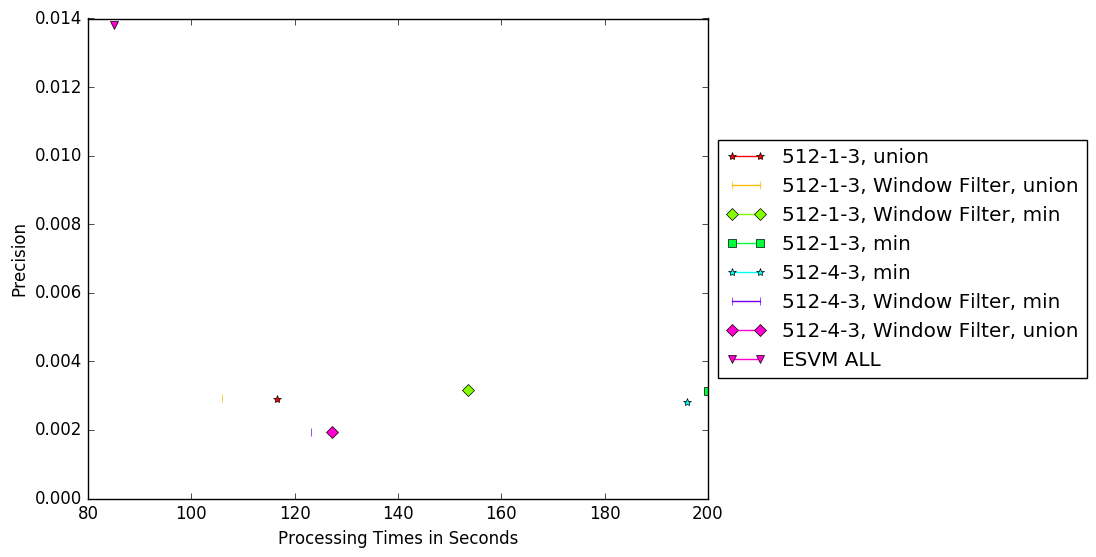
\includegraphics[width=0.7\linewidth]{images/val_t_vs_p-ALL}
\caption{Performance versus search time (2500 images)}
\label{fig:val_t_vs_p-ALL}
\end{figure}


\chapter{Conclusion}

The experimental results showed that the total query time can be reduced to a reasonable low amount, even if the queried database actually represents codebooks at every pixel with several hundred entries. Nevertheless, one of the bases of the algorithm (the codebooks) does not seem to provide the desired performances. One of the reasons may be the loss of the information about the exact locations and the sizes of the input feature patches. Another reason could be that the reduction of the 775 dimensional features to a codebook, shadows the essential information which actually represents the class of the query image. As the currently used system is unsupervised at the database creation, no information is available for the feature extraction nor which feature patch sizes should be included in a codebook. Furthermore, some of the experimental results indicate that smaller image parts with less feature patches get lost. This is based on the fact that a higher amount of features, which add up, would produce a higher profile codebook compared to a lower amount of features. Approaches like ExemplarSVM, which operate directly on the feature descriptors have to define the similarity between the descriptors themselves, whilst the presented approach has a higher dependency on the sorting of the describtors into the codebook bins. This means a sort of similarity assignment is required to preserve the performance of approaches, which do not use this additional layer.

The presented approach contains some promising parts (for example the ability to precompute a whole image database and extract arbitrary codebooks at query time), but cannot compete with algorithms like ExemplarSVM. Nevertheless, additional optimizations in terms of program code structure could reduce the query time even further, and therefore could be used as a filter algorithm to reduce the effort for more accurate algorithms.

\chapter{Outlook}

The next generations of the framework could have further speed and memory usage improvements by using code optimizations, as the current framework is developed to compare different approaches and replace different parts. Also, further experiments with the codebook approach could increase the detection performance. Possible improvements could be done in the separation of the input patches based on their sizes, while different feature pyramids could be created to get a broader range of input patches, which get combined into the database. The current method of constructing the codebook entries could be changed to allow fuzzy assignments and to use a normalization to get higher profiles even if only a small amount of patches are available. Further improvements to the loading and accessing of the database entries could be done by introducing hash tables instead or with the kd-Tree model, which would speed up the accessing time even more.

Another approach, which tries to go in the opposite direction, would be the usage of the integral image to estimate the existence of a searched object by triangulating it similarly to the currently used prefilter. This could maybe replace the sliding window approach and therefore decrease the effort dramatically.

Improvements compared to other algorithms based on hardware improvements would possibly only arise in terms of memory and file space. As the integral images could be used without the need of complicated data structures, individual entries could therefore be accessed in linear time.


\ifcomplete
% Schlagwortverzeichnis (Index)
\printindex

%\printglossaries

% Literaturverzeichnis
\singlespacing
%\bibliographystyle{alphadin}
%\bibliography{bibtex}
\printbibliography
%\nocite{*} % include all bibs
%
% Eidesstattliche Erklärung
\chapter*{Eidesstattliche Erklärung}
\markboth{Eidesstattliche Erklärung}{Eidesstattliche Erklärung}
% Eintrag in das Inhaltsverzeichnis 
\addcontentsline{toc}{chapter}{Eidesstattliche Erklärung}

Ich versichere, dass ich die vorstehende Arbeit selbständig verfasst und hierzu keine anderen als die angegebenen Hilfsmittel verwendet habe. Alle Stellen der Arbeit die wörtlich oder sinngemäß aus fremden Quellen entnommen wurden, sind als solche kenntlich gemacht.\\\\
\noindent
Die Arbeit wurde bisher in gleicher oder ähnlicher Form in keinem anderen Studiengang als Prüfungsleistung vorgelegt oder an anderer Stelle veröffentlicht.\\\\
\noindent
Ich bin mir bewusst, dass eine falsche Erklärung rechtliche Folgen haben kann.

%\vspace*{1.5cm} \par
%\line(1,0){200} \par
%\docOrt, den  \docAbgabedatum ~~\docVorname~\docNachname

\vspace*{1.5cm}
\begin{tabular}{@{}ll}
\line(1,0){150} & \line(1,0){150}\\ 
Ort, Datum & Unterschrift \\
\end{tabular} 


\pretocmd{\chapter}{%
  \clearpage
  \pagenumbering{arabic}%
  \renewcommand*{\thepage}{\thechapter-\arabic{page}}%
}{}{}
\begin{appendices}
% Hier können Anhaenge angefuegt werden
\chapter{Framework}

\section{Configuration Parameters}

%\begin{table}
\begin{longtable}{%
|%
p{0.2\textwidth}%
|%
>{\raggedright\arraybackslash}%
p{0.135\textwidth}%
|%
>{\raggedright\arraybackslash}%
p{0.135\textwidth}%
|%
>{\raggedright\arraybackslash}%
p{0.4\textwidth}%
|%
}
\hline \textbf{Parameter} & \textbf{Possible values} & \textbf{Default} & \textbf{Description} \\ 
\hline
\hline class & A PASCAL class & bicycle & Specifies the class to restrict the bounding boxes to \\ 
\hline parts & $x \in \mathbb{N} \textbackslash 0$ & 4 & Number of parts per window \\ 
\hline clusters & $x \in \mathbb{N} \textbackslash 0$ & 1000 & Number of k-Means clusters to use \\ 
\hline integrals\allowbreak\_scale\allowbreak\_factor & $x \in \mathbb{R}, 0 < x \le 1$ & 1 & Specifies the percentage to which a integral image should be downsampled to \\ 
\hline stream\allowbreak\_max & $x \in \mathbb{N} \textbackslash 0$ & 100 & Maximum amount of images used from a PASCAL stream \\ 
\hline stream\allowbreak\_name & Any string & query & Name of the PASCAL stream to read images from \\ 
\hline codebook\allowbreak\_type & double, single & double & Internal datatype of the codebooks \\ 
\hline codebook\allowbreak\_scales\allowbreak\_count & $x \in \mathbb{N} \textbackslash 0$ & 3 & Amount of scale ranges in which integral images will be split into \\ 
\hline nonmax\allowbreak\_type\allowbreak\_min & true, false & true & Specifies if $\frac{\text{area}(A \cap B)}{\min(\text{area}(A), \text{area}(B))}$ or $\frac{\text{area}(A \cap B)}{\text{area}(A \cup B)}$ should be used for a non-maximum suppression \\ 
\hline use\allowbreak\_calibration & true, false & true & If true, a score calibration based on the query image is performed \\ 
\hline features\allowbreak\_per\allowbreak\_roi & $x \in \mathbb{R}, 0 < x$ & 2 & Amount of feature patches which have to exist per window axis \\ 
\hline query\allowbreak\_from\allowbreak\_integral & true, false & false & If true, the query codebooks will be retrieved from the image database instead of extracted from the query image \\ 
\hline default\allowbreak\_query\allowbreak\_file & An image id & 2008\allowbreak\_004363 & Used to automate the experiments instead of asking interactively for a query image \\ 
\hline default\allowbreak\_bounding\allowbreak\_box & [x, y, width, height] & Extracted from the PASCAL dataset & The bounding box of the query image part \\ 
\hline use\allowbreak\_libsvm\allowbreak\_classification & true, false & true & If true, the \verb|svmpredict| function is used to classify the database codebooks. Otherwise a custom implementation is used \\ 
\hline expand\allowbreak\_bboxes & true, false & true & Expands the bounding boxes by $\frac{1}{2}$ of the average feature patch size \\ 
\hline naiive\allowbreak\_integral\allowbreak\_backend & true, false & true & Specifies to use full integral images without any memory optimization techniques \\ 
\hline window\allowbreak\_margin & $x \in \mathbb{N} \textbackslash 0$ & 10 & Amount of pixels each window is shifted during the sliding window generation  \\ 
\hline max\allowbreak\_window\allowbreak\_scales & $x \in \mathbb{N} \textbackslash 0$ & 10 & Maximum amount of times a scaling is performed during the sliding window generation \\ 
\hline min\allowbreak\_window\allowbreak\_size & $x \in \mathbb{R}, 0 < x \le 1$ & 0.5 & Required percentage of a window area which has to be placed over an image (windows are getting clipped at the image boundaries)\\
\hline window\allowbreak\_generation\allowbreak\_relative\allowbreak\_move & $x \in \mathbb{R}$ & 0 & Percentage of its size a window should move during sliding window (0 means fixed window\allowbreak\_margin pixels) \\
\hline max\allowbreak\_window\allowbreak\_image\allowbreak\_ratio & $x \in \mathbb{R}, 0 < x \le 1$ & 1.0 & Maximum allowed size of a window in relation to the image \\
\hline use\allowbreak\_kdtree & true, false & false & Enables the kd-Tree storage backend \\ 
\hline integral\allowbreak\_backend\allowbreak\_overwrite & true, false & false & Enables the integral matrix reconstruction via overwriting the bottom right values \\ 
\hline integral\allowbreak\_backend\allowbreak\_sum & true, false & false & Enables the integral matrix reconstruction via summing up the bottom right values \\ 
\hline integral\allowbreak\_backend\allowbreak\_matlab\allowbreak\_sparse & true, false & false & Enables the \MATLAB sparse storage backend \\ 
\hline precalced\allowbreak\_windows & true, false & false & Disables integral images and precalculates codebooks in a sliding window manner \\ 
\hline inverse\allowbreak\_search & true, false & false & Use the information of integral images to reduce the amount of windows generated. \\
\hline memory\allowbreak\_cache & true, false & true & Reuse already loaded databases and negative codebooks (useful for development) \\
\hline use\allowbreak\_threading & true, false & true & Enables the use of the parallel toolbox \\
\hline window\allowbreak\_prefilter & true, false & false & Prefilter the windows even further to reduce the amount of searched windows \\
\hline fisher\allowbreak\_backend & true, false & false & Use fisher vectors instead of k-means clusters (experimental as it is not practical) \\
\hline
\caption{Configuration parameters for the part retrieval framework}
\label{tab:configuration_framework}
\end{longtable}
%\end{table}


\section{Data Structures}
\label{apx:data_structures}

\begin{verbatim}
feature
    .all_scales         -> Scale factors used in the feature
                           pyramid
    .curid              -> ID of the image
    .objectid           -> Index of the object
    .feature_type       -> Extracted with a mask or not
    .I_size             -> Size of the input image
    .X                  -> The features itself
    .M                  -> The gradient
    .scales             -> The map between feature and scale
    .bbs                -> Patch bounding boxes
    .window2feature     -> List of sliding windows
    .area               -> Area of which the features were 
                           extracted
    .distVec            -> LDA distance vector
    .deletedFeatures    -> Removed features during filtering

integral
    .I                  -> The integral image itself
    .I_size             -> The size of the full integral image
    .curid              -> The ID of the source image
    .scale_factor       -> The factor of which the integral image
                           was shrinked
    .max_size           -> The maximum size of the patches used
                           inside the integral
    .min_size           -> The minimum size of the patches used
                           inside the integral
    .tree               -> kd-Tree representation
    .scores             -> The codebook entries
    .idx                -> The indices of the codebook entries
    .coords             -> The coordinates of the codebook
                           entries
    .small_tree         -> kd-Tree without the codebook entries

codebook
    .I                  -> The codebook itself
    .curid              -> The image were the codebook comes from
    .size               -> The size of the window

cluster
    .centroids                 -> The centroids of the k-means
    .codebookSize              -> The number of clusters/codebook
                                  dimensions
    .feature2codebook          -> function to get a codebook from
                                  a feature
    .feature2codebookintegral  -> function to get an integral image
                                  from a list of features

svm_model
    .model              -> The underlying implementation
        .SVs            -> Support vectors from libsvm
        .sv_coef        -> Coefficents from libsvm
        .rho            -> Rho from libsvm
    .curid              -> ID of the trained image
    .codebook           -> Used positive codebook
    .cb_size            -> Size of the codebook
    .classify           -> function to score a list of codebooks
\end{verbatim}

%TODO API?
%\section{API}
%
\subsection{DEMO}

Demo implementation

\paragraph{Syntax:} \verb|demo(train, ...)|

Inputs:

\begin{tabular}{|l|p{5cm}|}
\hline
\textbf{Name} & \textbf{Description} \\
\hline \hline \\
train & boolean to indicate the creation of a image database. Default: false  \\ \hline
Name & Value pairs to override the default configuration  \\ \hline
\end{tabular}

\subsection{GENERATECLUSTER}

Generate a cluster model

\paragraph{Syntax:} \verb|cluster_model = generateCluster(params)|

Inputs:

\begin{tabular}{|l|p{5cm}|}
\hline
\textbf{Name} & \textbf{Description} \\
\hline \hline \\
params & Configuration parameters  \\ \hline
\end{tabular}
Outputs:

\begin{tabular}{|l|p{5cm}|}
\hline
\textbf{Name} & \textbf{Description} \\
\hline \hline \\
cluster\_model & The model  \\ \hline
\end{tabular}

\subsection{GETIMAGEDB}

Generate or load the image database

\paragraph{Syntax:} \verb|database = getImageDB(params, cluster_model)|

Inputs:

\begin{tabular}{|l|p{5cm}|}
\hline
\textbf{Name} & \textbf{Description} \\
\hline \hline \\
cluster\_model & The model for codebook generation  \\ \hline
params & Configuration parameters  \\ \hline
\end{tabular}
Outputs:

\begin{tabular}{|l|p{5cm}|}
\hline
\textbf{Name} & \textbf{Description} \\
\hline \hline \\
database & The database of integral images  \\ \hline
\end{tabular}

\subsection{GETSVM}

Train or load a exemplar SVM

\paragraph{Syntax:} \verb|svm_models = getSVM(params, cluster_model)|

Inputs:

\begin{tabular}{|l|p{5cm}|}
\hline
\textbf{Name} & \textbf{Description} \\
\hline \hline \\
cluster\_model & The model to generate codebooks  \\ \hline
parms & Configuration parameters  \\ \hline
\end{tabular}
Outputs:

\begin{tabular}{|l|p{5cm}|}
\hline
\textbf{Name} & \textbf{Description} \\
\hline \hline \\
svm\_models & SVM model struct  \\ \hline
\end{tabular}

\subsection{SEARCHINTERACTIVE}

Do a complete interactive database searchAsks the user for a image in the dataset image path.Allows to mark a ROI to search forStores results in the results/queries subdirectories

\paragraph{Syntax:} \verb|searchInteractive(params, cluster_model)|

Inputs:

\begin{tabular}{|l|p{5cm}|}
\hline
\textbf{Name} & \textbf{Description} \\
\hline \hline \\
cluster\_model & The model to generate codebooks  \\ \hline
params & Configuration parameters  \\ \hline
\end{tabular}

\subsection{SEARCHDATABASE}

Search the image database with the given SVM modelsStores results in the results/queries subdirectories

\paragraph{Syntax:} \verb|results = searchDatabase(params, database, svm_models, fit_params, roi)|

Inputs:

\begin{tabular}{|l|p{5cm}|}
\hline
\textbf{Name} & \textbf{Description} \\
\hline \hline \\
svm\_models & Struct array of svm models  \\ \hline
roi & The region of interest [x\_{min}, y\_{min}, x\_{max}, y\_{max}]  \\ \hline
params & Configuration parameters  \\ \hline
fit\_params & Gaussian curve 2D Vectors to adjust the SVM scores [$\mu$, $\sigma$]  \\ \hline
database & The image database as struct array of integral codebook images  \\ \hline
\end{tabular}
Outputs:

\begin{tabular}{|l|p{5cm}|}
\hline
\textbf{Name} & \textbf{Description} \\
\hline \hline \\
results & Cell array of results. Fields: curid, img, patch, score  \\ \hline
\end{tabular}

\subsection{SEARCHDATABASE}

Search the image database with the given SVM modelsStores results in the results/queries subdirectories

\paragraph{Syntax:} \verb|results = searchDatabase(params, database, svm_models, fit_params, roi)|

Inputs:

\begin{tabular}{|l|p{5cm}|}
\hline
\textbf{Name} & \textbf{Description} \\
\hline \hline \\
svm\_models & Struct array of svm models  \\ \hline
roi & The region of interest [x\_{min}, y\_{min}, x\_{max}, y\_{max}]  \\ \hline
params & Configuration parameters  \\ \hline
fit\_params & Gaussian curve 2D Vectors to adjust the SVM scores [$\mu$, $\sigma$]  \\ \hline
database & The image database as struct array of integral codebook images  \\ \hline
\end{tabular}
Outputs:

\begin{tabular}{|l|p{5cm}|}
\hline
\textbf{Name} & \textbf{Description} \\
\hline \hline \\
results & Cell array of results. Fields: curid, img, patch, score  \\ \hline
\end{tabular}

\subsection{CALIBRATE\_FIT}

Estimates the gaussian parameters for the given svm models

\paragraph{Syntax:} \verb|fit_params = calibrate_fit(params, svm_models, query_file, cluster_model)|

Inputs:

\begin{tabular}{|l|p{5cm}|}
\hline
\textbf{Name} & \textbf{Description} \\
\hline \hline \\
svm\_models & The SVM models  \\ \hline
cluster\_model & The model to generate the codebooks  \\ \hline
params & Configuration parameters  \\ \hline
query\_file & A pascal stream containing the file used to train the SVM  \\ \hline
\end{tabular}
Outputs:

\begin{tabular}{|l|p{5cm}|}
\hline
\textbf{Name} & \textbf{Description} \\
\hline \hline \\
fit\_params & Nx2 matrix of gaussian parameters. N: number of SVM models, Gaussian Parameters: [$\mu$, $\sigma$]  \\ \hline
\end{tabular}

\subsection{CALIBRATE\_RHO}

Tries to readjust the rho of the given SVM models to obtain better scores

\paragraph{Syntax:} \verb|rhos = calibrate_rho(params, svm_models, query_file, cluster_model, ground_truths)|

Inputs:

\begin{tabular}{|l|p{5cm}|}
\hline
\textbf{Name} & \textbf{Description} \\
\hline \hline \\
svm\_models & The SVM models  \\ \hline
cluster\_model & The model to generate the codebooks  \\ \hline
ground\_truths & Nx4 Matrix of bounding boxes inside the query image (e.g. the ROI)  \\ \hline
params & Configuration parameters  \\ \hline
query\_file & A pascal stream containing the file used to train the SVM  \\ \hline
\end{tabular}
Outputs:

\begin{tabular}{|l|p{5cm}|}
\hline
\textbf{Name} & \textbf{Description} \\
\hline \hline \\
rhos & Mx1 vector of new rhos. M: number of SVM models  \\ \hline
\end{tabular}

\subsection{CONVERT\_SERIALIZE}

Creates a corresponding file with toggled serialization

\paragraph{Syntax:} \verb|convert_serialize(filename)|

Inputs:

\begin{tabular}{|l|p{5cm}|}
\hline
\textbf{Name} & \textbf{Description} \\
\hline \hline \\
filename & The file to invert  \\ \hline
\end{tabular}

\subsection{GET\_DEFAULT\_CONFIGURATION}

returns a default configuration

\paragraph{Syntax:} \verb|params = get_default_configuration()|

Outputs:

\begin{tabular}{|l|p{5cm}|}
\hline
\textbf{Name} & \textbf{Description} \\
\hline \hline \\
params & The default configuration  \\ \hline
\end{tabular}

\subsection{GET\_CODEBOOKS}

Get integral codebooks from given features

\paragraph{Syntax:} \verb|codebooks = get_codebooks(params, features, cluster_model)|

Inputs:

\begin{tabular}{|l|p{5cm}|}
\hline
\textbf{Name} & \textbf{Description} \\
\hline \hline \\
features & A feature struct array. Required Fields: curid, X, bbs, window2feature  \\ \hline
cluster\_model & A model from get\_cluster  \\ \hline
params & Configuration struct  \\ \hline
\end{tabular}
Outputs:

\begin{tabular}{|l|p{5cm}|}
\hline
\textbf{Name} & \textbf{Description} \\
\hline \hline \\
codebooks & A struct array with fields: I, curid, size  \\ \hline
\end{tabular}

\subsection{GET\_CODEBOOK\_INTEGRALS}

Get integral codebooks from given features

\paragraph{Syntax:} \verb|integrals = get_codebook_integrals(params, features, cluster_model, roi_size)|

Inputs:

\begin{tabular}{|l|p{5cm}|}
\hline
\textbf{Name} & \textbf{Description} \\
\hline \hline \\
features & A feature struct array. Required Fields: curid, X, bbs, I\_size, scales  \\ \hline
cluster\_model & A model from get\_cluster  \\ \hline
params & Configuration struct  \\ \hline
roi\_size & Size of the query part  \\ \hline
\end{tabular}
Outputs:

\begin{tabular}{|l|p{5cm}|}
\hline
\textbf{Name} & \textbf{Description} \\
\hline \hline \\
integrals & A struct array with fields: I, I\_size, curid, scale\_factor,max\_size, min\_size, tree,scores, idx, coords  \\ \hline
\end{tabular}

\subsection{GET\_CACHE\_BASEDIR}

Gets and creates the cache dir

\paragraph{Syntax:} \verb|basedir = get_cache_basedir(params, create_dir)|

Inputs:

\begin{tabular}{|l|p{5cm}|}
\hline
\textbf{Name} & \textbf{Description} \\
\hline \hline \\
create\_dir & Boolean to indicate the automatic creation of the dir  \\ \hline
params & Configuration struct  \\ \hline
\end{tabular}
Outputs:

\begin{tabular}{|l|p{5cm}|}
\hline
\textbf{Name} & \textbf{Description} \\
\hline \hline \\
basedir & The cache dir  \\ \hline
\end{tabular}

\subsection{GET\_CACHE\_NAME}

Gets the cache filename

\paragraph{Syntax:} \verb|cachename = get_cache_name(params, roi_size, create_dir)|

Inputs:

\begin{tabular}{|l|p{5cm}|}
\hline
\textbf{Name} & \textbf{Description} \\
\hline \hline \\
create\_dir & Boolean to indicate the automatic creation of the dir  \\ \hline
params & Configuration struct  \\ \hline
roi\_size & Vector containing the size of the roi or empty  \\ \hline
\end{tabular}
Outputs:

\begin{tabular}{|l|p{5cm}|}
\hline
\textbf{Name} & \textbf{Description} \\
\hline \hline \\
cachename & The cache file name  \\ \hline
\end{tabular}

\subsection{GET\_IMG\_CACHE\_NAME}

Gets the cache filename of a single image

\paragraph{Syntax:} \verb|imgcachename = get_img_cache_name(params, roi_size, create_dir)|

Inputs:

\begin{tabular}{|l|p{5cm}|}
\hline
\textbf{Name} & \textbf{Description} \\
\hline \hline \\
create\_dir & Boolean to indicate the automatic creation of the dir  \\ \hline
params & Configuration struct  \\ \hline
roi\_size & Vector containing the size of the roi or empty  \\ \hline
\end{tabular}
Outputs:

\begin{tabular}{|l|p{5cm}|}
\hline
\textbf{Name} & \textbf{Description} \\
\hline \hline \\
imgcachename & The cache file name  \\ \hline
\end{tabular}

\subsection{GET\_CLUSTER}

Clusters the given features with kmeans

\paragraph{Syntax:} \verb|model = get_cluster( params, features )|

Inputs:

\begin{tabular}{|l|p{5cm}|}
\hline
\textbf{Name} & \textbf{Description} \\
\hline \hline \\
features & The feature struct array (Required Fields: X)  \\ \hline
params & The configuration struct used for caching and profiling  \\ \hline
\end{tabular}
Outputs:

\begin{tabular}{|l|p{5cm}|}
\hline
\textbf{Name} & \textbf{Description} \\
\hline \hline \\
model & The computed model (Fields: centroids. Methods: feature2codebook(params, feature), feature2codebookintegral(params, feature))  \\ \hline
\end{tabular}

\subsection{FEATURE2CODEBOOK}

Calculates a codebook from a given feature struct

\paragraph{Syntax:} \verb|codebook = feature2codebook(params, feature, model)|

Inputs:

\begin{tabular}{|l|p{5cm}|}
\hline
\textbf{Name} & \textbf{Description} \\
\hline \hline \\
model & The cluster model. Required fields: centroids  \\ \hline
feature & The feature struct. Required fields: X, window2feature, bbs  \\ \hline
params & The configuration struct. Required fields: parts, codebook\_type, profile (if profiling is required)  \\ \hline
\end{tabular}
Outputs:

\begin{tabular}{|l|p{5cm}|}
\hline
\textbf{Name} & \textbf{Description} \\
\hline \hline \\
codebook & A NxM matrix. N: params.parts * size(centroids, 1), M: length(window2feature)  \\ \hline
\end{tabular}

\subsection{FEATURE2CODEBOOK}

Calculates a codebook integral from a given feature struct

\paragraph{Syntax:} \verb|codebook = feature2codebookintegral(params, feature, model)|

Inputs:

\begin{tabular}{|l|p{5cm}|}
\hline
\textbf{Name} & \textbf{Description} \\
\hline \hline \\
model & The cluster model. Required fields: centroids  \\ \hline
feature & The feature struct. Required fields: X, bbs, I\_size, scales  \\ \hline
params & The configuration struct. Required fields: codebook\_type, profile (if profiling is required)  \\ \hline
\end{tabular}
Outputs:

\begin{tabular}{|l|p{5cm}|}
\hline
\textbf{Name} & \textbf{Description} \\
\hline \hline \\
scales & A Cell of size S containing the associated scales.  \\ \hline
codebook & A SxNxWxH matrix. S: different scales, N: size(centroids, 1), W: I\_size(2), H: I\_size(1)  \\ \hline
\end{tabular}

\subsection{FEATURE2CODEBOOK}

Calculates a codebook integral from a given feature struct

\paragraph{Syntax:} \verb|codebook = feature2codebookintegral(params, feature, model)|

Inputs:

\begin{tabular}{|l|p{5cm}|}
\hline
\textbf{Name} & \textbf{Description} \\
\hline \hline \\
model & The cluster model. Required fields: centroids  \\ \hline
feature & The feature struct. Required fields: X, bbs, I\_size, scales  \\ \hline
params & The configuration struct. Required fields: codebook\_type, profile (if profiling is required)  \\ \hline
\end{tabular}
Outputs:

\begin{tabular}{|l|p{5cm}|}
\hline
\textbf{Name} & \textbf{Description} \\
\hline \hline \\
scales & A Cell of size S containing the associated scales.  \\ \hline
codebook & A SxNxWxH matrix. S: different scales, N: size(centroids, 1), W: I\_size(2), H: I\_size(1)  \\ \hline
\end{tabular}

\subsection{GET\_CODEBOOK\_FROM\_WINDOWS}

Get images codebooks from given features

\paragraph{Syntax:} \verb|images = get_codebook_from_windows(params, features, cluster_model, roi_size)|

Inputs:

\begin{tabular}{|l|p{5cm}|}
\hline
\textbf{Name} & \textbf{Description} \\
\hline \hline \\
features & A feature struct array. Required Fields: curid, X, bbs, I\_size, scales  \\ \hline
cluster\_model & A model from get\_cluster  \\ \hline
params & Configuration struct  \\ \hline
roi\_size & Size of the query part  \\ \hline
\end{tabular}
Outputs:

\begin{tabular}{|l|p{5cm}|}
\hline
\textbf{Name} & \textbf{Description} \\
\hline \hline \\
images & A struct array with fields: curid, scale\_factor, max\_size,min\_size, bboxes, codebooks, images  \\ \hline
\end{tabular}

\subsection{GET\_CACHE\_BASEDIR}

Gets and creates the cache dir

\paragraph{Syntax:} \verb|basedir = get_cache_basedir(params, create_dir)|

Inputs:

\begin{tabular}{|l|p{5cm}|}
\hline
\textbf{Name} & \textbf{Description} \\
\hline \hline \\
create\_dir & Boolean to indicate the automatic creation of the dir  \\ \hline
params & Configuration struct  \\ \hline
\end{tabular}
Outputs:

\begin{tabular}{|l|p{5cm}|}
\hline
\textbf{Name} & \textbf{Description} \\
\hline \hline \\
basedir & The cache dir  \\ \hline
\end{tabular}

\subsection{GET\_CACHE\_NAME}

Gets the cache filename

\paragraph{Syntax:} \verb|cachename = get_cache_name(params, roi_size, create_dir)|

Inputs:

\begin{tabular}{|l|p{5cm}|}
\hline
\textbf{Name} & \textbf{Description} \\
\hline \hline \\
create\_dir & Boolean to indicate the automatic creation of the dir  \\ \hline
params & Configuration struct  \\ \hline
roi\_size & Vector containing the size of the roi or empty  \\ \hline
\end{tabular}
Outputs:

\begin{tabular}{|l|p{5cm}|}
\hline
\textbf{Name} & \textbf{Description} \\
\hline \hline \\
cachename & The cache file name  \\ \hline
\end{tabular}

\subsection{GET\_IMG\_CACHE\_NAME}

Gets the cache filename of a single image

\paragraph{Syntax:} \verb|imgcachename = get_img_cache_name(params, roi_size, create_dir)|

Inputs:

\begin{tabular}{|l|p{5cm}|}
\hline
\textbf{Name} & \textbf{Description} \\
\hline \hline \\
create\_dir & Boolean to indicate the automatic creation of the dir  \\ \hline
params & Configuration struct  \\ \hline
roi\_size & Vector containing the size of the roi or empty  \\ \hline
\end{tabular}
Outputs:

\begin{tabular}{|l|p{5cm}|}
\hline
\textbf{Name} & \textbf{Description} \\
\hline \hline \\
imgcachename & The cache file name  \\ \hline
\end{tabular}

\subsection{GET\_IMAGE}

Loads a pascal image by its name

\paragraph{Syntax:} \verb|I = get_image( params, name )|

Inputs:

\begin{tabular}{|l|p{5cm}|}
\hline
\textbf{Name} & \textbf{Description} \\
\hline \hline \\
params & Configuration struct  \\ \hline
name & The image name  \\ \hline
\end{tabular}
Outputs:

\begin{tabular}{|l|p{5cm}|}
\hline
\textbf{Name} & \textbf{Description} \\
\hline \hline \\
I & The loaded image  \\ \hline
\end{tabular}

\subsection{GET\_FEATURES\_FROM\_STREAM}

Calculates HoG features from a given Pascal Stream

\paragraph{Syntax:} \verb|features = get_features_from_stream( params, stream )|

Inputs:

\begin{tabular}{|l|p{5cm}|}
\hline
\textbf{Name} & \textbf{Description} \\
\hline \hline \\
stream & A Pascal stream  \\ \hline
params & Configuration struct  \\ \hline
\end{tabular}
Outputs:

\begin{tabular}{|l|p{5cm}|}
\hline
\textbf{Name} & \textbf{Description} \\
\hline \hline \\
features & A feature struct array. Fields: curid, objectid,feature\_type, I\_size, X, M, scales, bbs, window2feature,area, all\_scales  \\ \hline
\end{tabular}

\subsection{EXTRACT\_QUERY\_CODEBOOK}

extracts a query codebook based on the configuration

\paragraph{Syntax:} \verb|query_codebooks = extract_query_codebook( params, cluster_model, query_file, roi_size )|

Inputs:

\begin{tabular}{|l|p{5cm}|}
\hline
\textbf{Name} & \textbf{Description} \\
\hline \hline \\
cluster\_model & Model representing the current clustering method  \\ \hline
params & Configuration struct  \\ \hline
roi\_size & Bounding box of the query part  \\ \hline
query\_file & Struct with information about the query file  \\ \hline
\end{tabular}
Outputs:

\begin{tabular}{|l|p{5cm}|}
\hline
\textbf{Name} & \textbf{Description} \\
\hline \hline \\
query\_codebooks & the resulting codebook  \\ \hline
\end{tabular}

\subsection{PREPARE\_FEATURES}

load or generate features for the given stream set

\paragraph{Syntax:} \verb|features = prepare_features(params, query_stream_set)|

Inputs:

\begin{tabular}{|l|p{5cm}|}
\hline
\textbf{Name} & \textbf{Description} \\
\hline \hline \\
query\_stream\_set & stream set containing the files to load  \\ \hline
params & Configuration struct  \\ \hline
\end{tabular}
Outputs:

\begin{tabular}{|l|p{5cm}|}
\hline
\textbf{Name} & \textbf{Description} \\
\hline \hline \\
features & struct array of features  \\ \hline
\end{tabular}

\subsection{GET\_FULL\_NEG\_MODEL}

Loads the negative model for whitened HoGs

\paragraph{Syntax:} \verb|neg_model = get_full_neg_model()|

Outputs:

\begin{tabular}{|l|p{5cm}|}
\hline
\textbf{Name} & \textbf{Description} \\
\hline \hline \\
neg\_model & The negative model  \\ \hline
\end{tabular}

\subsection{GET\_SVMS}

Get trained exemplar svms from given codebooks

\paragraph{Syntax:} \verb|svm_models = get_svms( params, query_codebooks, neg_codebooks )|

Inputs:

\begin{tabular}{|l|p{5cm}|}
\hline
\textbf{Name} & \textbf{Description} \\
\hline \hline \\
neg\_codebooks & Codebook struct array (Fields: I) or NxM matrix. N: Num codebooks, M: Codebook size  \\ \hline
params & Configuration struct  \\ \hline
query\_codebooks & A codebook struct array. Required Fields: I, size, curid  \\ \hline
\end{tabular}
Outputs:

\begin{tabular}{|l|p{5cm}|}
\hline
\textbf{Name} & \textbf{Description} \\
\hline \hline \\
svm\_models & Struct array of svm models. Fields: cb\_size, codebook, curid, model  \\ \hline
\end{tabular}

\subsection{ADJUST\_SCORES}

adjusts scores based on given gaussian fit parametersScores will applied on a gaussian curve. The curve is shifted by $3 * \sigma$and the resulting scores rescaled by $new\_scores * 2 - 1$

\paragraph{Syntax:} \verb|[ new_scores ] = adjust_scores( params, fit_params, scores )|

Inputs:

\begin{tabular}{|l|p{5cm}|}
\hline
\textbf{Name} & \textbf{Description} \\
\hline \hline \\
scores & Score vector to adjust  \\ \hline
params & Configuration parameters as struct  \\ \hline
fit\_params & 2D-Vector. [$\mu$, $\sigma$]  \\ \hline
\end{tabular}
Outputs:

\begin{tabular}{|l|p{5cm}|}
\hline
\textbf{Name} & \textbf{Description} \\
\hline \hline \\
new\_scores & Adjusted scores  \\ \hline
\end{tabular}

\subsection{GET\_RANGE\_FOR\_SCALE}

get the range of given scales

\paragraph{Syntax:} \verb|[ min_size, max_size ] = get_range_for_scale(params, current_scales)|

Inputs:

\begin{tabular}{|l|p{5cm}|}
\hline
\textbf{Name} & \textbf{Description} \\
\hline \hline \\
current\_scales & NxM matrix of scales  \\ \hline
params & Configuration struct  \\ \hline
\end{tabular}
Outputs:

\begin{tabular}{|l|p{5cm}|}
\hline
\textbf{Name} & \textbf{Description} \\
\hline \hline \\
max\_size & vector with N maximum values  \\ \hline
min\_size & vector with N minimum values  \\ \hline
\end{tabular}

\subsection{FILTER\_FEATURES}

Filters given featuresRemoves features with too little texture or which are too close to the negative mode of whitened features

\paragraph{Syntax:} \verb|features = filter_features(params, features)|

Inputs:

\begin{tabular}{|l|p{5cm}|}
\hline
\textbf{Name} & \textbf{Description} \\
\hline \hline \\
features & The feature struct array (Fields: X, M, distVec, scales, bbs, window2feature)  \\ \hline
params & The configuration struct. Used for profiling and caching  \\ \hline
\end{tabular}
Outputs:

\begin{tabular}{|l|p{5cm}|}
\hline
\textbf{Name} & \textbf{Description} \\
\hline \hline \\
features & The filtered feature struct array with new logical vector deletedFeatures  \\ \hline
\end{tabular}

\subsection{CALC\_CODEBOOKS}

Extracts codebooks and bounding boxes from a given image database

\paragraph{Syntax:} \verb|[ bboxes, codebooks, images ] = calc_codebooks(params, database, windows_bb, num_parts )|

Inputs:

\begin{tabular}{|l|p{5cm}|}
\hline
\textbf{Name} & \textbf{Description} \\
\hline \hline \\
windows\_bb & A Nx4 matrix of bounding boxes to to extract ($x\_{min}$, $y\_{min}$, $x\_{max}$, $y\_{max}$)  \\ \hline
num\_parts & (Even) number of segments a window should be divided to  \\ \hline
params & The configuration parameters, currently only required for profiling  \\ \hline
database & The image database as struct array with the fields I, curid and optionally scale\_factor  \\ \hline
\end{tabular}
Outputs:

\begin{tabular}{|l|p{5cm}|}
\hline
\textbf{Name} & \textbf{Description} \\
\hline \hline \\
images & A 1xN dimensional index vector for assigning codebooks to images  \\ \hline
bboxes & A Nx4 matrix of bounding boxes related to the extracted codebooks ($x\_{min}$, $y\_{min}$, $x\_{max}$, $y\_{max}$)  \\ \hline
codebooks & A Nx(M*num\_parts) matrix of M dimensional codebooks  \\ \hline
\end{tabular}

\subsection{EXPECTEDCODEBOOKS}

Tries to estimate the amount of codebooks extractedInternally used to preallocate the memory for speed

\paragraph{Syntax:} \verb|[expectedCodebookCount, codebookSize] = expectedCodebooks(database, windows_bb, num_parts)|

Inputs:

\begin{tabular}{|l|p{5cm}|}
\hline
\textbf{Name} & \textbf{Description} \\
\hline \hline \\
windows\_bb & A Nx4 matrix of bounding boxes to to extract  \\ \hline
num\_parts & (Even) number of segments a window should be divided to  \\ \hline
database & The image database as struct array with the field I  \\ \hline
\end{tabular}
Outputs:

\begin{tabular}{|l|p{5cm}|}
\hline
\textbf{Name} & \textbf{Description} \\
\hline \hline \\
expectedCodebookCount & Estimated number of codebooks which will be extracted  \\ \hline
codebookSize & Size of the resulting codebooks (M*num\_parts)  \\ \hline
\end{tabular}

\subsection{IS\_IN\_SCALE}

Tests if the requested sizes are within the a given scale

\paragraph{Syntax:} \verb|in_scale = is_in_scale(params, min_size, max_size, requested_size)|

Inputs:

\begin{tabular}{|l|p{5cm}|}
\hline
\textbf{Name} & \textbf{Description} \\
\hline \hline \\
max\_size & upper bound (or [] if lower bound is requested)  \\ \hline
params & Configuration struct  \\ \hline
min\_size & lower bound (or [] if upper bound is requested)  \\ \hline
\end{tabular}
Outputs:

\begin{tabular}{|l|p{5cm}|}
\hline
\textbf{Name} & \textbf{Description} \\
\hline \hline \\
in\_scale & logic vector  \\ \hline
\end{tabular}

\subsection{CALC\_WINDOWS}

Calculates the windows wich have to be extracted in a sliding window approach

\paragraph{Syntax:} \verb|windows_bb = calc_windows(params, w, h, cbw, cbh, I )|

Inputs:

\begin{tabular}{|l|p{5cm}|}
\hline
\textbf{Name} & \textbf{Description} \\
\hline \hline \\
cbw & Smallest width of a window  \\ \hline
cbh & Smallest height of a window  \\ \hline
I & Optional test image to produce a intagral.avi file for visualization  \\ \hline
w & Width of the image  \\ \hline
params & Configuration struct  \\ \hline
h & Height of the image  \\ \hline
\end{tabular}
Outputs:

\begin{tabular}{|l|p{5cm}|}
\hline
\textbf{Name} & \textbf{Description} \\
\hline \hline \\
windows\_bb & Nx4 matrix of windows ($x\_{min}$, $y\_{min}$, $x\_{max}$, $y\_{max}$)  \\ \hline
\end{tabular}

\subsection{SPARSE\_CODEBOOK}

Matlab implementation of the reconstruction of a kd-Tree integral image

\paragraph{Syntax:} \verb|codebook = sparse_codebook(integral, x, y)|

Inputs:

\begin{tabular}{|l|p{5cm}|}
\hline
\textbf{Name} & \textbf{Description} \\
\hline \hline \\
x, y & Coordinate of requested codebook  \\ \hline
integral & An integral image with kd-Tree storage backend  \\ \hline
\end{tabular}
Outputs:

\begin{tabular}{|l|p{5cm}|}
\hline
\textbf{Name} & \textbf{Description} \\
\hline \hline \\
codebook & the reconstructed codebook  \\ \hline
\end{tabular}

\subsection{GETCODEBOOKSFROMINTEGRAL}

Extract codebooks from a single integral image

\paragraph{Syntax:} \verb|codebooks = getCodebooksFromIntegral(params, integral_img, bboxes, num_parts)|

Inputs:

\begin{tabular}{|l|p{5cm}|}
\hline
\textbf{Name} & \textbf{Description} \\
\hline \hline \\
bboxes & Mx4 Matrix of bounding boxes to extract  \\ \hline
num\_parts & (Even) number of segments to divide a single window into  \\ \hline
integral\_img & SxNxWxH Matrix. S: scales, N: Codebook Size, W: Width, H: Height  \\ \hline
params & Configuration struct  \\ \hline
\end{tabular}
Outputs:

\begin{tabular}{|l|p{5cm}|}
\hline
\textbf{Name} & \textbf{Description} \\
\hline \hline \\
codebooks & N2xSxM Matrix. N2: N*num\_parts  \\ \hline
\end{tabular}

\subsection{ESTIMATE\_FIT\_PARAMS}

Estimates parameters of a gaussian curveCan be used to adjust the scores

\paragraph{Syntax:} \verb|fit_params = estimate_fit_params( params, scores )|

Inputs:

\begin{tabular}{|l|p{5cm}|}
\hline
\textbf{Name} & \textbf{Description} \\
\hline \hline \\
scores & Score vector to fit to  \\ \hline
params & Configuration struct (currently not used)  \\ \hline
\end{tabular}
Outputs:

\begin{tabular}{|l|p{5cm}|}
\hline
\textbf{Name} & \textbf{Description} \\
\hline \hline \\
fit\_params & 2D-Vector of parameters [$\mu$, $\sigma$]  \\ \hline
\end{tabular}

\subsection{GETPARTS}

Calculates the segments of a window

\paragraph{Syntax:} \verb|[ xsteps, ysteps ] = getParts( minX, minY, maxX, maxY, num_parts)|

Inputs:

\begin{tabular}{|l|p{5cm}|}
\hline
\textbf{Name} & \textbf{Description} \\
\hline \hline \\
num\_parts & (Even) number of segments  \\ \hline
minY & Lowest y value  \\ \hline
maxY & Highest y value  \\ \hline
minX & Lowest x value  \\ \hline
maxX & Highest x value  \\ \hline
\end{tabular}
Outputs:

\begin{tabular}{|l|p{5cm}|}
\hline
\textbf{Name} & \textbf{Description} \\
\hline \hline \\
ysteps & Y offsets inside the bounding box [[from; to], ...] (2xnum\_parts Matrix)  \\ \hline
xsteps & X offsets inside the bounding box [[from; to], ...] (2xnum\_parts Matrix)  \\ \hline
\end{tabular}

\subsection{JOIN\_PART\_COVARIANCES}

Joins multiple small files into one matrix

\paragraph{Syntax:} \verb|neg_model = join_part_covariances(num_parts)|

Inputs:

\begin{tabular}{|l|p{5cm}|}
\hline
\textbf{Name} & \textbf{Description} \\
\hline \hline \\
num\_parts & Number of files to join  \\ \hline
\end{tabular}
Outputs:

\begin{tabular}{|l|p{5cm}|}
\hline
\textbf{Name} & \textbf{Description} \\
\hline \hline \\
neg\_model & the negative model for whitened HoGs  \\ \hline
\end{tabular}

\subsection{REDUCE\_MATCHES}

Reduces the amount of detected matches with a non-max suppression

\paragraph{Syntax:} \verb|[bbox, scores, idx] = reduce_matches(params, bbox, scores)|

Inputs:

\begin{tabular}{|l|p{5cm}|}
\hline
\textbf{Name} & \textbf{Description} \\
\hline \hline \\
bbox & Nx4 matrix of bounding boxes [x, y, w, h]  \\ \hline
params & Configuration parameters  \\ \hline
scores & N dimensional vector of scores  \\ \hline
\end{tabular}
Outputs:

\begin{tabular}{|l|p{5cm}|}
\hline
\textbf{Name} & \textbf{Description} \\
\hline \hline \\
bbox & New bounding boxes  \\ \hline
idx & Mapping between input and output (index vector)  \\ \hline
scores & New scores  \\ \hline
\end{tabular}

\subsection{GETHOGSINSIDEBOX}

Restrict calculated HoGs to a given mask

\paragraph{Syntax:} \verb|[X, W, M, offsets, uus, vvs, scales] = getHogsInsideBox(t, I, mask, params)|

Inputs:

\begin{tabular}{|l|p{5cm}|}
\hline
\textbf{Name} & \textbf{Description} \\
\hline \hline \\
I & Source image of features  \\ \hline
mask & logical mask to restrict features (same size as source image)  \\ \hline
t & Feature pyramid  \\ \hline
params & Configuration parameters  \\ \hline
\end{tabular}
Outputs:

\begin{tabular}{|l|p{5cm}|}
\hline
\textbf{Name} & \textbf{Description} \\
\hline \hline \\
W & wavelet  \\ \hline
uus & Patch positions  \\ \hline
offsets & Patch offsets  \\ \hline
M & Gradient  \\ \hline
vvs & Patch positions  \\ \hline
X & Features (Nx775)  \\ \hline
scales & Patch scales  \\ \hline
\end{tabular}

\subsection{WHITEN\_FEATURES}

Transforms HoG features into whitened HoGs

\paragraph{Syntax:} \verb|features = whiten_features( params, features )|

Inputs:

\begin{tabular}{|l|p{5cm}|}
\hline
\textbf{Name} & \textbf{Description} \\
\hline \hline \\
features & Feature struct array. Required Fields: X, M  \\ \hline
params & Configuration struct  \\ \hline
\end{tabular}
Outputs:

\begin{tabular}{|l|p{5cm}|}
\hline
\textbf{Name} & \textbf{Description} \\
\hline \hline \\
features & Whitened feature struct array. New Field: distVec  \\ \hline
\end{tabular}

\subsection{MERGE\_STRUCTS}

Merges multiple structs togetherFields of the first struct gets overriden by the second, the third, ....

\paragraph{Syntax:} \verb|result = merge_structs(struct1, struct2, ...)|

Outputs:

\begin{tabular}{|l|p{5cm}|}
\hline
\textbf{Name} & \textbf{Description} \\
\hline \hline \\
result & The merged struct  \\ \hline
\end{tabular}

\subsection{PROFILE\_STEP}

Logs an execution traceLogs where it was called and which time elapsed since the profiling start

\paragraph{Syntax:} \verb|params = profile_log( params )|

Inputs:

\begin{tabular}{|l|p{5cm}|}
\hline
\textbf{Name} & \textbf{Description} \\
\hline \hline \\
params & A configuration struct produced by profile\_start  \\ \hline
\end{tabular}
Outputs:

\begin{tabular}{|l|p{5cm}|}
\hline
\textbf{Name} & \textbf{Description} \\
\hline \hline \\
params & The input struct with updated profile.steps field (not required for subsequential calls)  \\ \hline
\end{tabular}

\subsection{MAKE\_SOUND}

Plays a soundtrack to get attentionCould be used to signal the end of a computation or the presence of an error

\paragraph{Syntax:} \verb|make_sound( finished )|

Inputs:

\begin{tabular}{|l|p{5cm}|}
\hline
\textbf{Name} & \textbf{Description} \\
\hline \hline \\
finished & Boolean, specifies if a gong (false) or a handel (true) should be played  \\ \hline
\end{tabular}

\subsection{SAVE\_EX}

Advanced wrapper around saveProvides status information and to serialize the variables with hlp\_serialize

\paragraph{Syntax:} \verb|save_ex(filename, save_args, ...)|

Inputs:

\begin{tabular}{|l|p{5cm}|}
\hline
\textbf{Name} & \textbf{Description} \\
\hline \hline \\
save\_args & Variadic arguments for matlabs save function  \\ \hline
filename & The file to save to  \\ \hline
\end{tabular}

\subsection{PARSE\_KEYWORDS}

Parses a list of arguments into a structRequires arguments of the form Keyword1, Value1, Keyword2, Value2, ...

\paragraph{Syntax:} \verb|keywords = parse_keywords(input_args, allowed_keywords)|

Inputs:

\begin{tabular}{|l|p{5cm}|}
\hline
\textbf{Name} & \textbf{Description} \\
\hline \hline \\
input\_args & Cell array of input arguments (e.g. varargin)  \\ \hline
allowed\_keywords & Optional cell array of allowed keywords  \\ \hline
\end{tabular}
Outputs:

\begin{tabular}{|l|p{5cm}|}
\hline
\textbf{Name} & \textbf{Description} \\
\hline \hline \\
keywords & Struct of keyword, value pairs  \\ \hline
\end{tabular}

\subsection{LOAD\_EX}

Advanced load wrapperPrints status information and allows to load files serialized with hlp\_deserializeBehaves exactly like matlabs load function

\paragraph{Syntax:} \verb|out = load_ex(filename, load_arg, ...)|

Inputs:

\begin{tabular}{|l|p{5cm}|}
\hline
\textbf{Name} & \textbf{Description} \\
\hline \hline \\
load\_arg & Optional, variadic arguments for matlabs load function  \\ \hline
filename & File to load  \\ \hline
\end{tabular}
Outputs:

\begin{tabular}{|l|p{5cm}|}
\hline
\textbf{Name} & \textbf{Description} \\
\hline \hline \\
serialized & optional boolean indicating the load of a serialized var  \\ \hline
out & optional struct containing the loaded variables  \\ \hline
\end{tabular}

\subsection{STRUCT2STR}

converts a struct into a printable string

\paragraph{Syntax:} \verb|str = struct2str(in, recursive)|

Inputs:

\begin{tabular}{|l|p{5cm}|}
\hline
\textbf{Name} & \textbf{Description} \\
\hline \hline \\
recursive & boolean to indicate a recursive print  \\ \hline
in & the struct to print  \\ \hline
\end{tabular}
Outputs:

\begin{tabular}{|l|p{5cm}|}
\hline
\textbf{Name} & \textbf{Description} \\
\hline \hline \\
str & String containing a text representation of the struct  \\ \hline
\end{tabular}

\subsection{PROFILE\_STOP}

Stops the profilingRecords the total execution time during the profiling

\paragraph{Syntax:} \verb|profile_stop( params )|

Inputs:

\begin{tabular}{|l|p{5cm}|}
\hline
\textbf{Name} & \textbf{Description} \\
\hline \hline \\
params & The configuration struct processed by profile\_start  \\ \hline
\end{tabular}

\subsection{PROFILE\_START}

Starts an execution traceupdates the given configuration struct by adding a profile field with subfieldsrecords the start time.

\paragraph{Syntax:} \verb|params = profile_start( params )|

Inputs:

\begin{tabular}{|l|p{5cm}|}
\hline
\textbf{Name} & \textbf{Description} \\
\hline \hline \\
params & A configuration struct with a configured dataset (dataset.localdir field is required)  \\ \hline
\end{tabular}
Outputs:

\begin{tabular}{|l|p{5cm}|}
\hline
\textbf{Name} & \textbf{Description} \\
\hline \hline \\
params & The updated struct. Required for profile\_log and profile\_stop calls  \\ \hline
\end{tabular}

\subsection{ALLOC\_STRUCT\_ARRAY}

Allocates a struct array of given size with given fieldsSorts fieldnames to be in line with matlabs save -struct

\paragraph{Syntax:} \verb|array = alloc_struct_array( size, field, ... )|

Inputs:

\begin{tabular}{|l|p{5cm}|}
\hline
\textbf{Name} & \textbf{Description} \\
\hline \hline \\
field & Variable number of fields to be contained in the array  \\ \hline
size & The requested size of the struct array (vector possible)  \\ \hline
\end{tabular}
Outputs:

\begin{tabular}{|l|p{5cm}|}
\hline
\textbf{Name} & \textbf{Description} \\
\hline \hline \\
array & The 1xsize struct array  \\ \hline
\end{tabular}

\subsection{SET\_LOG\_LEVEL}

set current log level

\paragraph{Syntax:} \verb|set_log_level(lvl)|

Inputs:

\begin{tabular}{|l|p{5cm}|}
\hline
\textbf{Name} & \textbf{Description} \\
\hline \hline \\
lvl & set the current log level  \\ \hline
\end{tabular}

\subsection{GET\_LOG\_LEVEL}

get current log level as string

\paragraph{Syntax:} \verb|lvl = get_log_level()|

Outputs:

\begin{tabular}{|l|p{5cm}|}
\hline
\textbf{Name} & \textbf{Description} \\
\hline \hline \\
lvl & get the current log level  \\ \hline
\end{tabular}

\subsection{DEBG}

log a debug message

\paragraph{Syntax:} \verb|debg(fmt, ..., [addprefix], [addnewline])|

Inputs:

\begin{tabular}{|l|p{5cm}|}
\hline
\textbf{Name} & \textbf{Description} \\
\hline \hline \\
addprefix & optional boolean to indicate if the prefix should be prepended  \\ \hline
addnewline & optional boolean to indicate if a new line should be appended  \\ \hline
fmt & Message to log. Formatting available  \\ \hline
\end{tabular}

\subsection{ERR}

log a error message

\paragraph{Syntax:} \verb|err(fmt, ..., [addprefix], [addnewline])|

Inputs:

\begin{tabular}{|l|p{5cm}|}
\hline
\textbf{Name} & \textbf{Description} \\
\hline \hline \\
addprefix & optional boolean to indicate if the prefix should be prepended  \\ \hline
addnewline & optional boolean to indicate if a new line should be appended  \\ \hline
fmt & Message to log. Formatting available  \\ \hline
\end{tabular}

\subsection{LOG\_FILE}

gets or sets the log file

\paragraph{Syntax:} \verb|fname = log_file([filename])|

Inputs:

\begin{tabular}{|l|p{5cm}|}
\hline
\textbf{Name} & \textbf{Description} \\
\hline \hline \\
filename & optional filename to set  \\ \hline
\end{tabular}
Outputs:

\begin{tabular}{|l|p{5cm}|}
\hline
\textbf{Name} & \textbf{Description} \\
\hline \hline \\
fname & current logfile  \\ \hline
\end{tabular}

\subsection{LOG\_LEVEL}

gets or sets the log level

\paragraph{Syntax:} \verb|ll = log_level([level])|

Inputs:

\begin{tabular}{|l|p{5cm}|}
\hline
\textbf{Name} & \textbf{Description} \\
\hline \hline \\
level & optional log level to set  \\ \hline
\end{tabular}
Outputs:

\begin{tabular}{|l|p{5cm}|}
\hline
\textbf{Name} & \textbf{Description} \\
\hline \hline \\
ll & current log level  \\ \hline
\end{tabular}

\subsection{WARN}

log a warning message

\paragraph{Syntax:} \verb|warn(fmt, ..., [addprefix], [addnewline])|

Inputs:

\begin{tabular}{|l|p{5cm}|}
\hline
\textbf{Name} & \textbf{Description} \\
\hline \hline \\
addprefix & optional boolean to indicate if the prefix should be prepended  \\ \hline
addnewline & optional boolean to indicate if a new line should be appended  \\ \hline
fmt & Message to log. Formatting available  \\ \hline
\end{tabular}

\subsection{INFO}

log a info message

\paragraph{Syntax:} \verb|info(fmt, ..., [addprefix], [addnewline])|

Inputs:

\begin{tabular}{|l|p{5cm}|}
\hline
\textbf{Name} & \textbf{Description} \\
\hline \hline \\
addprefix & optional boolean to indicate if the prefix should be prepended  \\ \hline
addnewline & optional boolean to indicate if a new line should be appended  \\ \hline
fmt & Message to log. Formatting available  \\ \hline
\end{tabular}

\subsection{LOG\_MSG}

internal logging function

\paragraph{Syntax:} \verb|log_msg(newfmt, fmt, ..., [addprefix], [addnewline])|

Inputs:

\begin{tabular}{|l|p{5cm}|}
\hline
\textbf{Name} & \textbf{Description} \\
\hline \hline \\
newfmt & Prefix format  \\ \hline
addnewline & optional boolean to indicate if a new line should be appended  \\ \hline
fmt & Message to log. Formatting available  \\ \hline
addprefix & optional boolean to indicate if the prefix should be prepended  \\ \hline
\end{tabular}

\subsection{SUCC}

log a success message

\paragraph{Syntax:} \verb|succ(fmt, ..., [addprefix], [addnewline])|

Inputs:

\begin{tabular}{|l|p{5cm}|}
\hline
\textbf{Name} & \textbf{Description} \\
\hline \hline \\
addprefix & optional boolean to indicate if the prefix should be prepended  \\ \hline
addnewline & optional boolean to indicate if a new line should be appended  \\ \hline
fmt & Message to log. Formatting available  \\ \hline
\end{tabular}

\subsection{RECONSTRUCT\_MATRIX\_BY\_OVERWRITE}

reconstructs a given sparse matrix into a full integral image

\paragraph{Syntax:} \verb|outmatrix = reconstruct_matrix_by_overwrite(integral)|

Inputs:

\begin{tabular}{|l|p{5cm}|}
\hline
\textbf{Name} & \textbf{Description} \\
\hline \hline \\
integral & integral struct with fields scores, coords, I\_size  \\ \hline
\end{tabular}
Outputs:

\begin{tabular}{|l|p{5cm}|}
\hline
\textbf{Name} & \textbf{Description} \\
\hline \hline \\
outmatrix & Expanded integral matrix  \\ \hline
\end{tabular}

\subsection{SPARSE\_CODEBOOK\_INTEGRAL}

calculates a codebook entry from a kd-Tee based integral image

\paragraph{Syntax:} \verb|codebook = sparse_codebook_integral(integral, queryX, queryY)|

Inputs:

\begin{tabular}{|l|p{5cm}|}
\hline
\textbf{Name} & \textbf{Description} \\
\hline \hline \\
x, y & x and y coordinates (2 elements per vector)  \\ \hline
integral & integral struct with fields tree.x and tree.y. Scores mustnot be summed up beforehand.  \\ \hline
\end{tabular}
Outputs:

\begin{tabular}{|l|p{5cm}|}
\hline
\textbf{Name} & \textbf{Description} \\
\hline \hline \\
codebook & Codebook vector  \\ \hline
\end{tabular}

\subsection{RECONSTRUCT\_MATRIX}

reconstructs a given sparse matrix into a full integral image

\paragraph{Syntax:} \verb|outmatrix = reconstruct_matrix(inmatrix)|

Inputs:

\begin{tabular}{|l|p{5cm}|}
\hline
\textbf{Name} & \textbf{Description} \\
\hline \hline \\
inmatrix & DxWxH Matrix with changed cells filled, everything else 0  \\ \hline
\end{tabular}
Outputs:

\begin{tabular}{|l|p{5cm}|}
\hline
\textbf{Name} & \textbf{Description} \\
\hline \hline \\
outmatrix & The same matrix but expanded into a integral matrix.Input matrix is reused for speed  \\ \hline
\end{tabular}

\subsection{SPARSE\_CODEBOOK}

calculates a codebook entry from a kd-Tee based integral image

\paragraph{Syntax:} \verb|codebook = sparse_codebook(integral, queryX, queryY)|

Inputs:

\begin{tabular}{|l|p{5cm}|}
\hline
\textbf{Name} & \textbf{Description} \\
\hline \hline \\
queryX, queryY & requested coordinates  \\ \hline
integral & integral struct with fields tree.x and tree.y. Scores mustnot be summed up beforehand.  \\ \hline
\end{tabular}
Outputs:

\begin{tabular}{|l|p{5cm}|}
\hline
\textbf{Name} & \textbf{Description} \\
\hline \hline \\
codebook & Codebook vector  \\ \hline
\end{tabular}

\subsection{RECONSTRUCT\_MATRIX\_BY\_SUM}

reconstructs a given sparse matrix into a full integral image

\paragraph{Syntax:} \verb|outmatrix = reconstruct_matrix_by_sum(integral)|

Inputs:

\begin{tabular}{|l|p{5cm}|}
\hline
\textbf{Name} & \textbf{Description} \\
\hline \hline \\
integral & integral struct with fields scores, coords, I\_size. Scores mustnot be summed up beforehand.  \\ \hline
\end{tabular}
Outputs:

\begin{tabular}{|l|p{5cm}|}
\hline
\textbf{Name} & \textbf{Description} \\
\hline \hline \\
outmatrix & Expanded integral matrix  \\ \hline
\end{tabular}

\subsection{GET\_CURRENT\_SCALES\_BY\_INDEX}

get the current scales by an index

\paragraph{Syntax:} \verb|current_scales = get_current_scales_by_index(si, unique_scales, scale_sizes)|

Inputs:

\begin{tabular}{|l|p{5cm}|}
\hline
\textbf{Name} & \textbf{Description} \\
\hline \hline \\
si & index  \\ \hline
unique\_scales & available scales  \\ \hline
scale\_sizes & amount of scales per split  \\ \hline
\end{tabular}
Outputs:

\begin{tabular}{|l|p{5cm}|}
\hline
\textbf{Name} & \textbf{Description} \\
\hline \hline \\
current\_scales & unique list of scales  \\ \hline
\end{tabular}

\subsection{SORT\_CACHE\_FILES}

sort a list of cache files by sizes extracted by the given format

\paragraph{Syntax:} \verb|[files, sizes] = sort_cache_files(files, format)|

Inputs:

\begin{tabular}{|l|p{5cm}|}
\hline
\textbf{Name} & \textbf{Description} \\
\hline \hline \\
files & list of possible files  \\ \hline
format & format string to extract the sizes  \\ \hline
\end{tabular}
Outputs:

\begin{tabular}{|l|p{5cm}|}
\hline
\textbf{Name} & \textbf{Description} \\
\hline \hline \\
sizes & list of extracted sizes  \\ \hline
files & list of resorted files  \\ \hline
\end{tabular}

\subsection{FILTER\_FEATURE\_BY\_SCALE}

filters given features by a list of of given scales

\paragraph{Syntax:} \verb|filtered = filter_feature_by_scale(current_scales, feature)|

Inputs:

\begin{tabular}{|l|p{5cm}|}
\hline
\textbf{Name} & \textbf{Description} \\
\hline \hline \\
feature & feature struct  \\ \hline
current\_scales & Vector of possible scales  \\ \hline
\end{tabular}
Outputs:

\begin{tabular}{|l|p{5cm}|}
\hline
\textbf{Name} & \textbf{Description} \\
\hline \hline \\
filtered & logic vector  \\ \hline
\end{tabular}

\subsection{GET\_AVAILABLE\_SCALES}

get the available scales by this feature struct

\paragraph{Syntax:} \verb|[unique_scales, scale_sizes] = get_available_scales(params, feature)|

Inputs:

\begin{tabular}{|l|p{5cm}|}
\hline
\textbf{Name} & \textbf{Description} \\
\hline \hline \\
feature & feature struct  \\ \hline
params & Configuration struct  \\ \hline
\end{tabular}
Outputs:

\begin{tabular}{|l|p{5cm}|}
\hline
\textbf{Name} & \textbf{Description} \\
\hline \hline \\
scale\_sizes & amount of scales per split  \\ \hline
unique\_scales & unique list of scales  \\ \hline
\end{tabular}

\subsection{FILTER\_CACHE\_FILES}

filters a list of cache files based on the best matching query size

\paragraph{Syntax:} \verb|filename = filter_cache_files(params, files, sizes, requested_size)|

Inputs:

\begin{tabular}{|l|p{5cm}|}
\hline
\textbf{Name} & \textbf{Description} \\
\hline \hline \\
sizes & corresponding sizes  \\ \hline
files & list of possible files  \\ \hline
params & Configuration struct  \\ \hline
requested\_size & size of query part  \\ \hline
\end{tabular}
Outputs:

\begin{tabular}{|l|p{5cm}|}
\hline
\textbf{Name} & \textbf{Description} \\
\hline \hline \\
filename & path of best matching file  \\ \hline
\end{tabular}

\subsection{GET\_CURRENT\_SCALES\_BY\_SIZE}

get the current scales by a query size

\paragraph{Syntax:} \verb|current_scales = get_current_scales_by_size(params, unique_scales, scale_sizes, roi_size)|

Inputs:

\begin{tabular}{|l|p{5cm}|}
\hline
\textbf{Name} & \textbf{Description} \\
\hline \hline \\
scale\_sizes & amount of scales per split  \\ \hline
roi\_sizes & query size  \\ \hline
params & Configuration struct  \\ \hline
unique\_scales & available scales  \\ \hline
\end{tabular}
Outputs:

\begin{tabular}{|l|p{5cm}|}
\hline
\textbf{Name} & \textbf{Description} \\
\hline \hline \\
current\_scales & unique list of scales  \\ \hline
\end{tabular}

\subsection{GET\_POSSIBLE\_CACHE\_FILES}

get all possible cache files based on a format string

\paragraph{Syntax:} \verb|files = get_possible_cache_files(cachename)|

Inputs:

\begin{tabular}{|l|p{5cm}|}
\hline
\textbf{Name} & \textbf{Description} \\
\hline \hline \\
cachename & format string to search for. Replaces %d by *  \\ \hline
\end{tabular}
Outputs:

\begin{tabular}{|l|p{5cm}|}
\hline
\textbf{Name} & \textbf{Description} \\
\hline \hline \\
files & list of possible files  \\ \hline
\end{tabular}


\chapter{Experiments}
\section{Dataset 50}
\label{apx:images50}
\VerbatimInput{../sources/thesis2/data/bicycle_database.txt}

%% wild gesammelte ideen/texte


\section{Extracting HOG based on PASCAL bounding boxes}

\section{steps nn}
\begin{enumerate}
	\item extract hog for all bicycle and car training images with bounding box
	\item cluster features with 3000 kmeans cluster
	\item extract hog for all bicycle test images with bounding box
	\item generate codebook for each window in each image \ref{codebook_calculation_alg}
	\item calculate euclidean distance between codebooks
	\item iterate over all test images and print with N nearest images
\end{enumerate}
	
\section{steps nn-iter}
\begin{enumerate}
	\item extract hog for all bicycle and car training images with bounding box
	\item cluster features with 3000 kmeans cluster
	\item extract hog for all bicycle test images with bounding box
	\item generate codebook for each window in each image \ref{codebook_calculation_alg}
	\item calculate euclidean distance between codebooks
	\item iterate over all test images and print with N nearest images\label{nn_iter_loop_start}
	\item remove codebook entries if not shared by other N images
	\item restart with \ref{nn_iter_loop_start} till no changes
\end{enumerate}

\section{steps svm}
\begin{enumerate}
	\item extract hog for all bicycle training images with sliding window
	\item randomly discard 55\% of windows per image to fit into memory
	\item cluster features with 3000 kmeans cluster
	\item extract hog for all bicycle training images with bounding boxes as positives
	\item extract hog for all bicycle training images except bounding boxes as negatives
	\item assign features by nearest neighbor to clusters to generate codebook \ref{codebook_calculation_alg}
	\item train exemplar svm for each positive
	\item extract hog for all bicycle test images with sliding window
	\item generate codebook for each window in each image
	\item assign label for each window with each trained svm
\end{enumerate}

\begin{eqnarray}
codebook_k : \text{element at position }k\text{ in codebook} \\
f_i : \text{feature }i\text{ of window or image} \\
C_k : \text{cluster }k \\
d_{ik} : \text{distance of feature }i\text{ to cluster }k \\
a_{ik} : \begin{cases}
1 & \text{if }f_i\text{ belongs to }C_k \\
0 & \text{otherwise}
\end{cases} \\
codebook_k = \sum_{i=1}^N \frac{a_{ik}}{d_{ik}}
\label{codebook_calculation_alg}
\end{eqnarray}

\section{steps nn-fisher}
\begin{enumerate}
	\item extract hog for all bicycle and car training images with bounding box
	\item cluster features with 128 gmm cluster
	\item extract hog for all bicycle test images with bounding box
	\item calculate fishervector for every image
	\item calculate euclidean distance between codebooks
	\item iterate over all test images and print with N nearest images
\end{enumerate}
\end{appendices}

\fi

\end{document}
